\documentclass[11pt,a4paper]{article}

% Pacotes essenciais
\usepackage[utf8]{inputenc}
\usepackage[T1]{fontenc}
\usepackage{lmodern}
\usepackage[portuguese]{babel}
\usepackage{graphicx}
\usepackage{amsmath}
\usepackage{amsfonts}
\usepackage{amssymb}
\usepackage{float}
\usepackage{caption}
\usepackage{subcaption}
\usepackage{xcolor}
\usepackage{colortbl}
\usepackage{fancyhdr}
\usepackage{geometry}
\usepackage{titlesec}
\usepackage{lipsum}
\usepackage[alf]{abntex2cite}
\usepackage{booktabs}
\usepackage{array}
\usepackage{enumitem}
\usepackage{tikz}
\usetikzlibrary{shapes.geometric}
\usepackage[hidelinks]{hyperref}

% Definição das cores
\definecolor{headercolor}{HTML}{b11116}
\definecolor{secondarycolor}{HTML}{3a5461}

% Configuração da página
\geometry{
    a4paper,
    top=2.8cm,
    bottom=2.5cm,
    left=2.5cm,
    right=2.5cm,
    headheight=1.2cm,
    headsep=0.5cm
}

% Configuração do cabeçalho
\pagestyle{fancy}
\fancyhf{}
\renewcommand{\headrulewidth}{0pt}
\renewcommand{\footrulewidth}{0.5pt}

\fancyhead[L]{%
    \begin{tikzpicture}[remember picture, overlay]
        \fill[headercolor] (current page.north west) rectangle ([yshift=-1.2cm]current page.north east);
        \node[anchor=west, inner sep=0pt] at ([xshift=1cm, yshift=-0.6cm]current page.north west) 
            {
\includegraphics[height=0.8cm]{imgs/base/fatec-rgt.png}};
        \node[anchor=east, inner sep=0pt] at ([xshift=-1cm, yshift=-0.6cm]current page.north east) 
            {
\includegraphics[height=0.9cm]{imgs/base/cps-logo.png}};
        \node[anchor=east, inner sep=0pt] at ([xshift=-2.8cm, yshift=-0.6cm]current page.north east) 
            {
\includegraphics[height=1.05cm]{imgs/base/governo-sp-secretaria-logo.png}};
    \end{tikzpicture}
}

\fancyfoot[L]{\footnotesize\textcolor{secondarycolor}{Faculdade de Tecnologia do Estado de São Paulo\\ fatecregistro.cps.sp.gov.br}}
\fancyfoot[R]{\thepage}

% Configuração dos títulos das seções
\titleformat{\section}
    {\normalfont\large\bfseries\color{secondarycolor}}
    {\thesection}{1em}{}

\titleformat{\subsection}
    {\normalfont\normalsize\bfseries\color{secondarycolor}}
    {\thesubsection}{1em}{}

\begin{document}

% ===== CAPA =====
\begin{titlepage}
    \centering
    
    % Logos no topo
    \begin{tikzpicture}[remember picture, overlay]
        \fill[headercolor] (current page.north west) rectangle ([yshift=-1.2cm]current page.north east);
        \node[anchor=west, inner sep=0pt] at ([xshift=1cm, yshift=-0.6cm]current page.north west) 
            {
\includegraphics[height=0.8cm]{imgs/base/fatec-rgt.png}};
        \node[anchor=east, inner sep=0pt] at ([xshift=-1cm, yshift=-0.6cm]current page.north east) 
            {
\includegraphics[height=0.9cm]{imgs/base/cps-logo.png}};
        \node[anchor=east, inner sep=0pt] at ([xshift=-2.8cm, yshift=-0.6cm]current page.north east) 
            {
\includegraphics[height=1.05cm]{imgs/base/governo-sp-secretaria-logo.png}};
    \end{tikzpicture}
    
    \vspace*{3.5cm}
    
    % Nome da faculdade
    {\normalsize FACULDADE DE TECNOLOGIA DO ESTADO DE SÃO PAULO\par}
    \vspace{0.5cm}
    
    % Curso
    {\normalsize DESENVOLVIMENTO DE SOFTWARE MULTIPLATAFORMA\par}
    
    \vspace{4cm}
    
    % Artefatos do Projeto de Software
    {\normalsize ARTEFATOS DO PROJETO DE SOFTWARE\par}
    
    \vspace{0.3cm}
    
    % Nome do projeto
    {\normalsize Controle de Tráfego utilizando Câmeras Inteligentes, orientado por Visão Computacional\par}
    
    \vspace{3cm}
    
    % Autores
    {\normalsize
    Bruno de Lucca Soares Miranda\\
    Cristhian Hatzman Trigo\\
    João Paulo Goreri Rustichelli\\
    Marcelo Augusto Pedroso Martins\\
    Paulo Seiji Yamamoto Junior
    }
    
    \vfill
    
    % Rodapé
    {\small Registro -- SP\\
    2026}
    
\end{titlepage}

% Força o cabeçalho em todas as páginas
\pagestyle{fancy}

% ===== SUMÁRIO =====
\tableofcontents
\newpage

% ===== NOTA IMPORTANTE =====
\section*{Nota Importante sobre os Artefatos}

\noindent Este documento apresenta exemplos de como inserir os principais artefatos de um projeto de software. Todos os artefatos podem ser inseridos de duas formas:

\begin{enumerate}
    \item \textbf{Como imagens:} Criar os artefatos em ferramentas externas (Canva, Miro, Draw.io, Figma, etc.) e inserir como imagens PNG/JPG usando o comando \texttt{\textbackslash includegraphics}
    \item \textbf{Como código LaTeX:} Usar tabelas e diagramas TikZ diretamente no documento (exemplos fornecidos)
\end{enumerate}

\subsection*{Lista de Artefatos e suas Finalidades}

\begin{itemize}
    \item \textbf{CANVAS:} Modelo de negócio e estratégia
    \item \textbf{SWOT:} Análise estratégica de forças, fraquezas, oportunidades e ameaças
    \item \textbf{UX/UI:} Design de interface e experiência do usuário
    \item \textbf{Website:} Estrutura e especificações técnicas web
    \item \textbf{Diagramas UML:} Modelagem visual do sistema
    \item \textbf{DevOps:} Infraestrutura, automação e práticas de entrega contínua
\end{itemize}

\vspace{0.5cm}
\noindent\rule{\textwidth}{0.5pt}

\newpage

% ===== CANVAS =====
\section{CANVAS: Modelo de Negócio e Estratégia}

\begin{table}[H]
\centering
\caption{SmarTraffic -- Visão Geral}
\label{tab:canvas}
\small
\renewcommand{\arraystretch}{1.3}
\begin{tabular}{|>{\raggedright\arraybackslash}p{2.7cm}|>{\raggedright\arraybackslash}p{2.7cm}|>{\raggedright\arraybackslash}p{2.7cm}|>{\raggedright\arraybackslash}p{2.7cm}|>{\raggedright\arraybackslash}p{2.7cm}|}
\hline
\textbf{Parcerias Principais} & \textbf{Atividades Chave} & \textbf{Proposta de Valor} & \textbf{Relacionamento} & \textbf{Segmentos de Clientes} \\
\hline
DTI (câmeras), Secretaria de Trânsito, Engenheiros Eletricistas, Fornecedores de Câmeras IP, Empresas de infraestrutura urbana, Empresas de telecom, Fabricantes semafóricos
&
Desenvolver e treinar modelos de IA, Integrar IA com hardware de controle, Oferecer suporte técnico e manutenção, Atualizar modelos de IA periodicamente
&
Semáforo Inteligente que detecta veículos e pedestres em tempo real, Detecção de PCDs com tempo de travessia estendido, Reduzir congestionamentos, Aumentar segurança da via, Adaptar automaticamente o tempo do semáforo de acordo com o fluxo real, Criação de dados reais do fluxo
&
Período de testes em um cruzamento sem custo, Contrato de manutenção preventiva, Desconto para expansão para mais cruzamentos
&
Prefeituras municipais, Motoristas/Pedestres, Foco Inicial na cidade de Registro-SP \\
\hline
\textbf{Fontes de Renda} & \textbf{Recursos Chave} & \textbf{Estrutura de Custos} & \multicolumn{2}{l|}{\textbf{Canais}} \\
\hline
Venda única (hardware + instalação), Assinatura mensal/anual (software + suporte), Capacitação da equipe da prefeitura para operar o sistema
&
Câmeras, Visão Computacional, Arduino
&
Implantação por cruzamento (hardware e instalação), Recorrentes (suporte e manutenção, atualização dos modelos de IA), Margem (venda do kit e assinatura mensal)
&
\multicolumn{2}{p{5.6cm}|}{Venda direta para prefeituras (licitação ou contrato direto), Instalação piloto em um cruzamento (parceria com a prefeitura local)} \\
\hline
\end{tabular}
\end{table}

% ===== SWOT =====
\section{SWOT: Análise Estratégica}

\begin{table}[H]
\centering
\caption{Análise SWOT do Projeto}
\label{tab:swot}
\begin{tabular}{|p{7.2cm}|p{7.2cm}|}
\hline
\multicolumn{2}{|c|}{\cellcolor{secondarycolor!20}\textbf{FATORES INTERNOS}} \\
\hline
\textbf{FORÇAS (Strengths)} & \textbf{FRAQUEZAS (Weaknesses)} \\
\hline
\begin{minipage}[t]{7cm}
\begin{itemize}
    \item Protótipo funcional de detecção com YOLOv8n (carros e pessoas)
    \item Comunicação Python $\to$ Arduino via serial (9600 baud) implementada
    \item Interface Flask + Socket.IO para monitoramento local
    \item Código aberto e reproduzível (pesos versionados no repositório)
    \item Alinhamento com ODS 9 e 11 (como objetivo, não resultado)
\end{itemize}
\end{minipage}
&
\begin{minipage}[t]{7cm}
\begin{itemize}
    \item Contagem por quadro $\neq$ veículos únicos (sem tracking)
    \item Sem ROI por via — não separa filas A e B
    \item Sem watchdog no Arduino — fallback depende do Python
    \item delay() bloqueante no firmware
    \item Comandos sem ACK estruturado (Python muda estado sem confirmação física)
    \item Flask sem autenticação e CORS aberto
    \item Métricas de eficiência ainda não medidas
\end{itemize}
\end{minipage}
\\
\hline
\multicolumn{2}{|c|}{\cellcolor{secondarycolor!20}\textbf{FATORES EXTERNOS}} \\
\hline
\textbf{OPORTUNIDADES (Opportunities)} & \textbf{AMEAÇAS (Threats)} \\
\hline
\begin{minipage}[t]{7cm}
\begin{itemize}
    \item Expansão para 4 aproximações e múltiplos cruzamentos
    \item Integração com AWS para histórico e processamento
    \item Dashboard de monitoramento para operadores de trânsito
    \item Atendimento de pedestres/PCD (escopo desejado, mecanismo a definir)
    \item Uso de rastreamento (tracking) para contagem única
\end{itemize}
\end{minipage}
&
\begin{minipage}[t]{7cm}
\begin{itemize}
    \item Falha de câmera/PC/serial sem fallback autônomo no controlador 
    \item Falso positivo/negativo do YOLO em cenas com oclusão
    \item Privacidade e LGPD na captura de pessoas
    \item Custo de implantação/manutenção 
    \item Dependência de documentação desatualizada para reprodução
\end{itemize}
\end{minipage}
\\
\hline
\end{tabular}
\end{table}

% ===== UX/UI =====
\section{UX/UI: Design de Interface e Experiência do Usuário}

UX (User Experience) e UI (User Interface) \cite{silva2025} são disciplinas complementares focadas em criar produtos digitais que sejam funcionais, acessíveis e agradáveis de usar.\footnote{Ferramentas populares para design UX/UI incluem Figma, Adobe XD, Sketch e InVision.} O UX concentra-se na experiência geral do usuário, enquanto o UI cuida dos elementos visuais e interativos.

\subsection{Como Inserir Mockups e Protótipos}

Os artefatos de UX/UI geralmente incluem wireframes, mockups e protótipos que podem ser inseridos como imagens:

\begin{figure}[H]
\centering
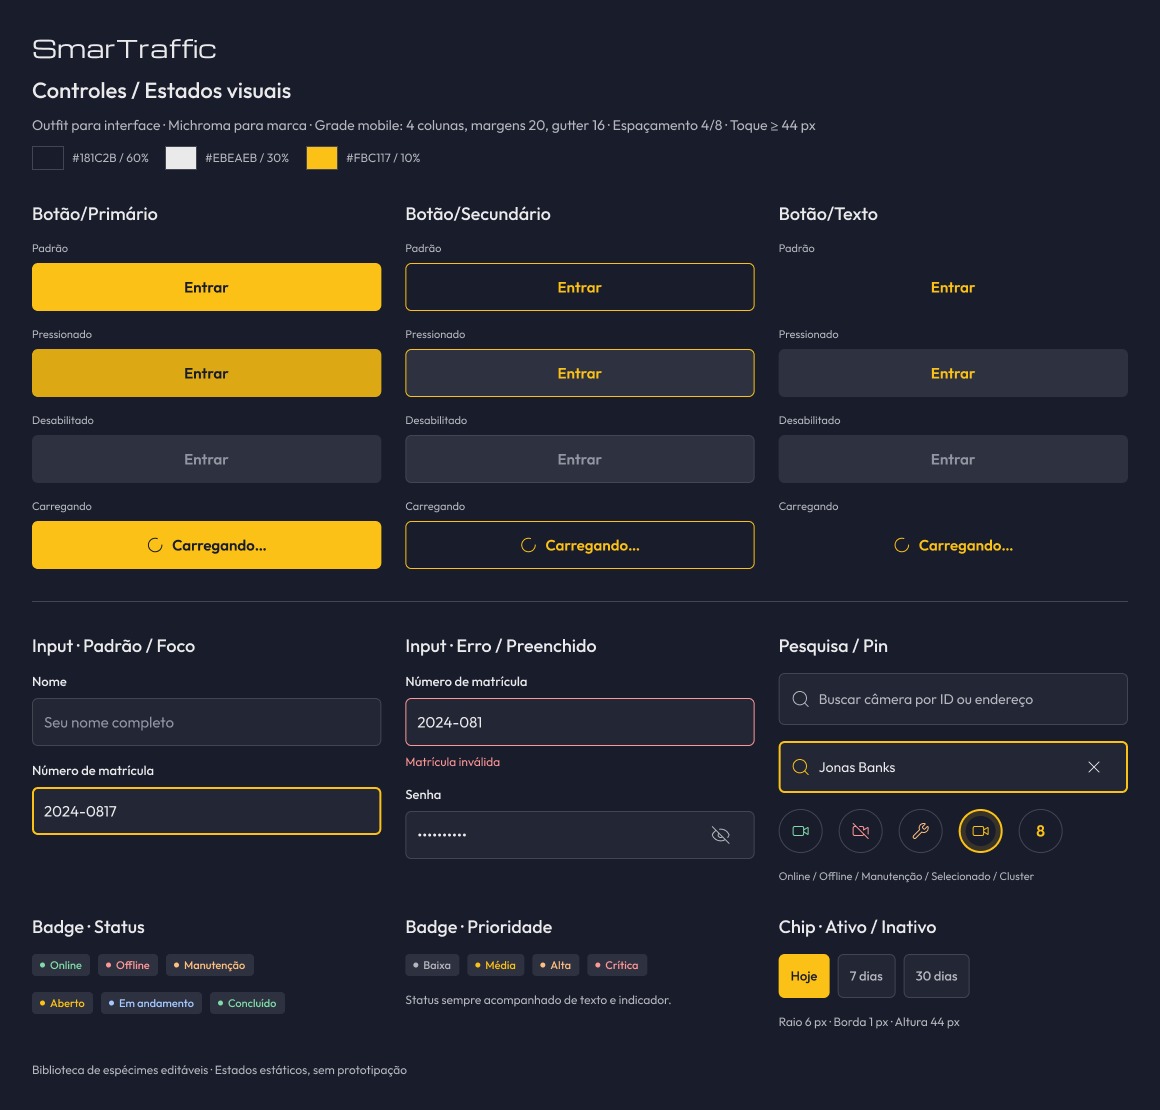
\includegraphics[width=\textwidth]{imgs/mobile/componentes-controles-e-estados.png}
\caption{Componentes de Controle e Estados}
\label{fig:website-controles}
\end{figure}

\begin{figure}[H]
\centering
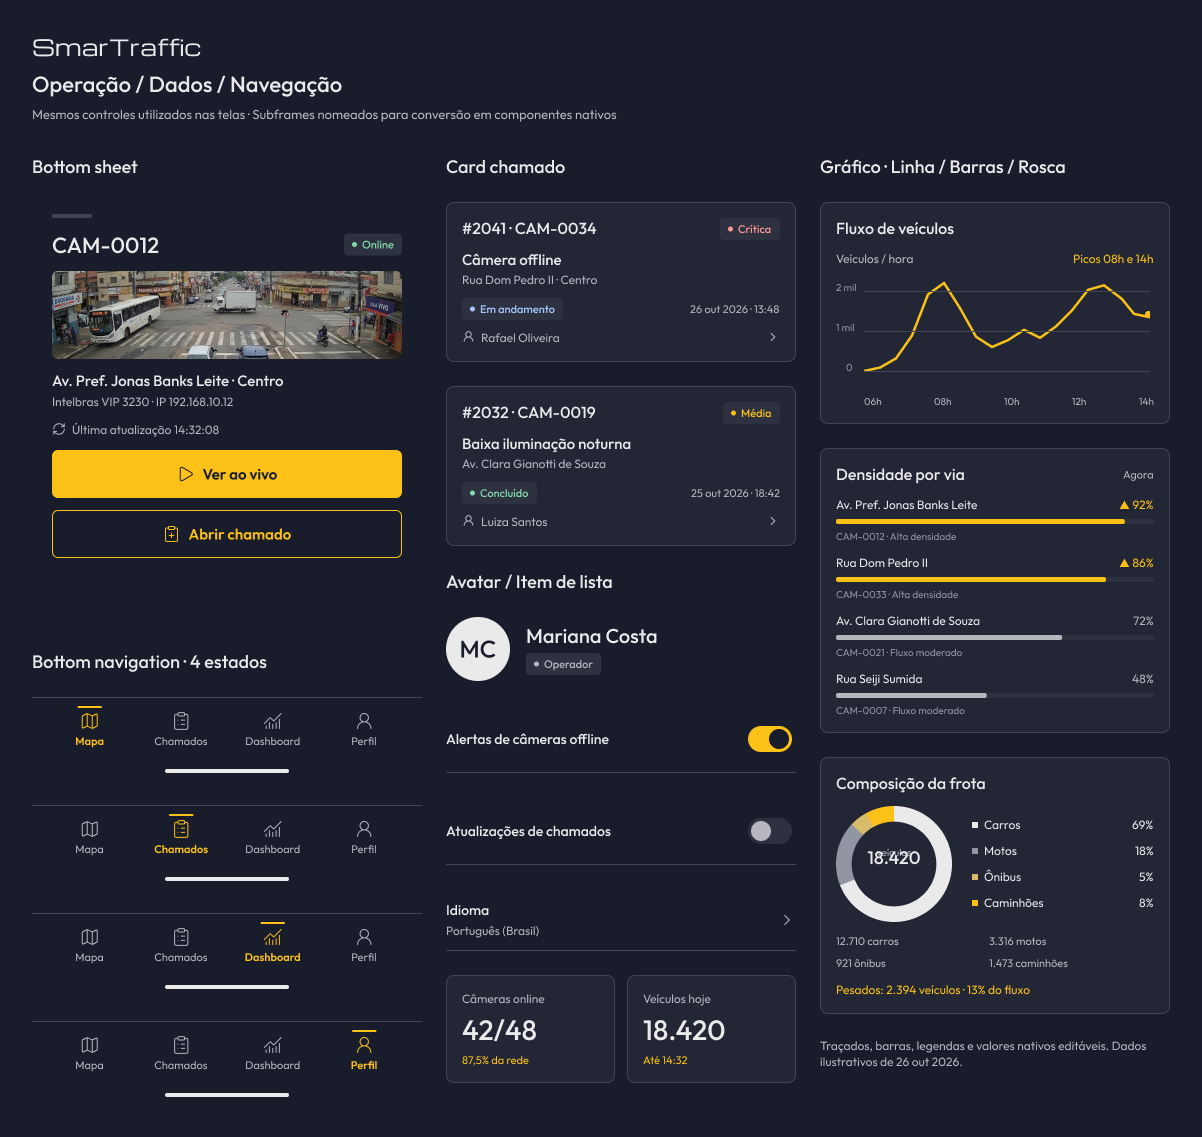
\includegraphics[width=\textwidth]{imgs/mobile/componentes-operacao-e-navegacao.png}
\caption{Componentes de Operacao e Estados}
\label{fig:website-operacao}
\end{figure}

\begin{figure}[H]
\centering
\begin{minipage}{0.45\textwidth}
    \centering
    \fbox{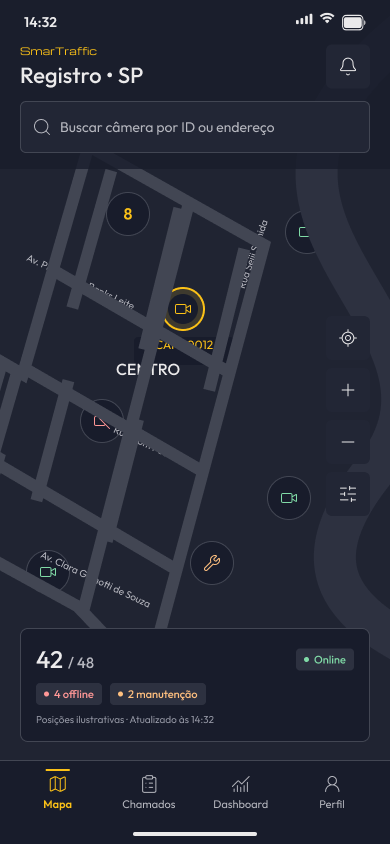
\includegraphics[width=0.9\textwidth]{imgs/mobile/02-home-mapa.png}}
    \label{fig:mobile1}
\end{minipage}
\hfill
\begin{minipage}{0.45\textwidth}
    \centering
    \fbox{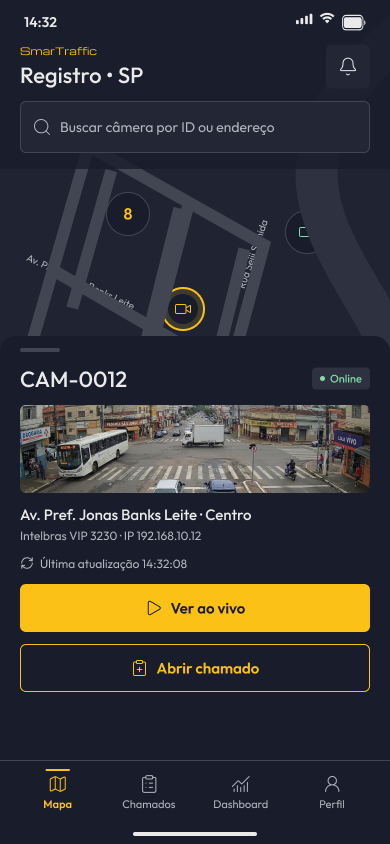
\includegraphics[width=0.9\textwidth]{imgs/mobile/02a-detalhe-da-camera.png}}
    \label{fig:mobile2}
\end{minipage}
\end{figure}

\begin{figure}[H]
\centering
\begin{minipage}{0.45\textwidth}
    \centering
    \fbox{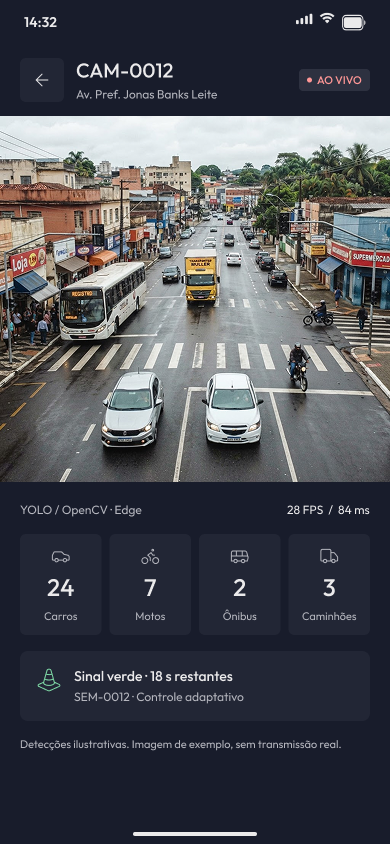
\includegraphics[width=0.9\textwidth]{imgs/mobile/02b-ao-vivo-deteccao-ilustrativa.png}}
    \label{fig:mobile3}
\end{minipage}
\hfill
\begin{minipage}{0.45\textwidth}
    \centering
    \fbox{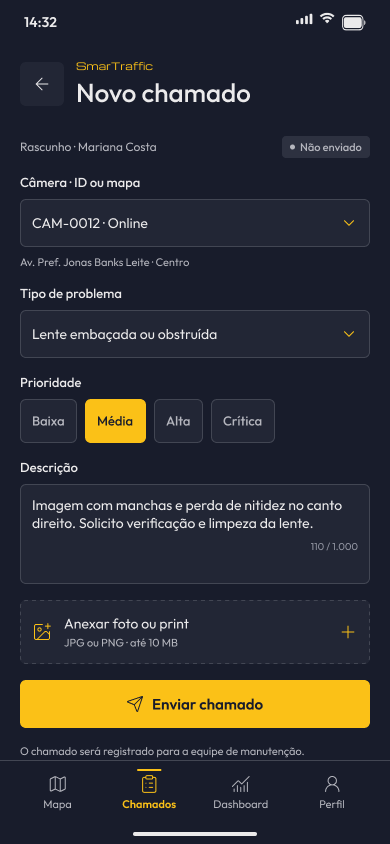
\includegraphics[width=0.9\textwidth]{imgs/mobile/04b-novo-chamado-rascunho-cam-0012.png}}
    \label{fig:mobile4}
\end{minipage}
\end{figure}

\subsection{Guia de Estilos}

É importante documentar o design system utilizado:

\begin{table}[H]
\centering
\caption{Paleta de Cores do Projeto}
\label{tab:cores}
\begin{tabular}{|l|c|l|l|}
\hline
\textbf{Elemento} & \textbf{Cor} & \textbf{Código HEX} & \textbf{Uso} \\
\hline
Primária & \colorbox[HTML]{181C2B}{\phantom{AAA}} & \#181C2B & Botões principais, destaques \\
Secundária & \colorbox[HTML]{EBEAEB}{\phantom{AAA}} & \#EBEAEB & Títulos, elementos secundários \\
Fundo & \colorbox[HTML]{FBC117}{\phantom{AAA}} & \#FBC117 & Background padrão \\
\hline
\end{tabular}
\end{table}

\begin{table}[H]
\centering
\caption{Paleta de Cores da Equipe}
\label{tab:cores}
\begin{tabular}{|l|c|l|l|}
\hline
\textbf{Elemento} & \textbf{Cor} & \textbf{Código HEX} & \textbf{Uso} \\
\hline
Primária & \colorbox[HTML]{0093FB}{\phantom{AAA}} & \#0093FB & Cor Principal \\
Secundária & \colorbox[HTML]{FE920A}{\phantom{AAA}} & \#FE920A & Cor Secundária \\
Fundo & \colorbox[HTML]{181C2B}{\phantom{AAA}} & \#181C2B & Cor Terciária \\
\hline
\end{tabular}
\end{table}

% ===== WEBSITE =====
\section{Website: Estrutura e Especificações Técnicas Web}

Esta seção documenta o website institucional/portfólio da equipe que desenvolveu a aplicação. O site da equipe serve para apresentar os membros, projetos realizados, competências e informações de contato.

\subsection{Mapa do Site da Equipe}

O mapa do site (sitemap) mostra a hierarquia e organização das páginas do website da equipe:

\begin{figure}[H]
\centering
\begin{tikzpicture}[
    level 1/.style={sibling distance=4cm, level distance=1.5cm},
    level 2/.style={sibling distance=2cm, level distance=1.5cm},
    every node/.style={rectangle, draw, rounded corners, 
                       fill=secondarycolor!20, 
                       text width=2.5cm, 
                       align=center,
                       font=\small}
]
\node {Syncro}
    child {node {Inicio/Home}
        child {node {Quem Somos?}}
    }
    child {node {Equipe}
        child {node {Geral}}
    }
    child {node {Tecnologias}
        child {node {Fluxo}}
    }
    child {node {Projeto}
        child {node {SmarTraffic}}
    };
    
\end{tikzpicture}
\caption{Estrutura de navegação do website da equipe}
\label{fig:sitemap-equipe}
\end{figure}

\subsection{Telas do Website da Equipe}

Para documentar as páginas do website da equipe:


\begin{figure}[H]
\centering

\includegraphics[width=\textwidth]{imgs/site_web/equipe/carrosel.jpeg}
\label{fig:website-carrosel}
\end{figure}

\begin{figure}[H]
\centering
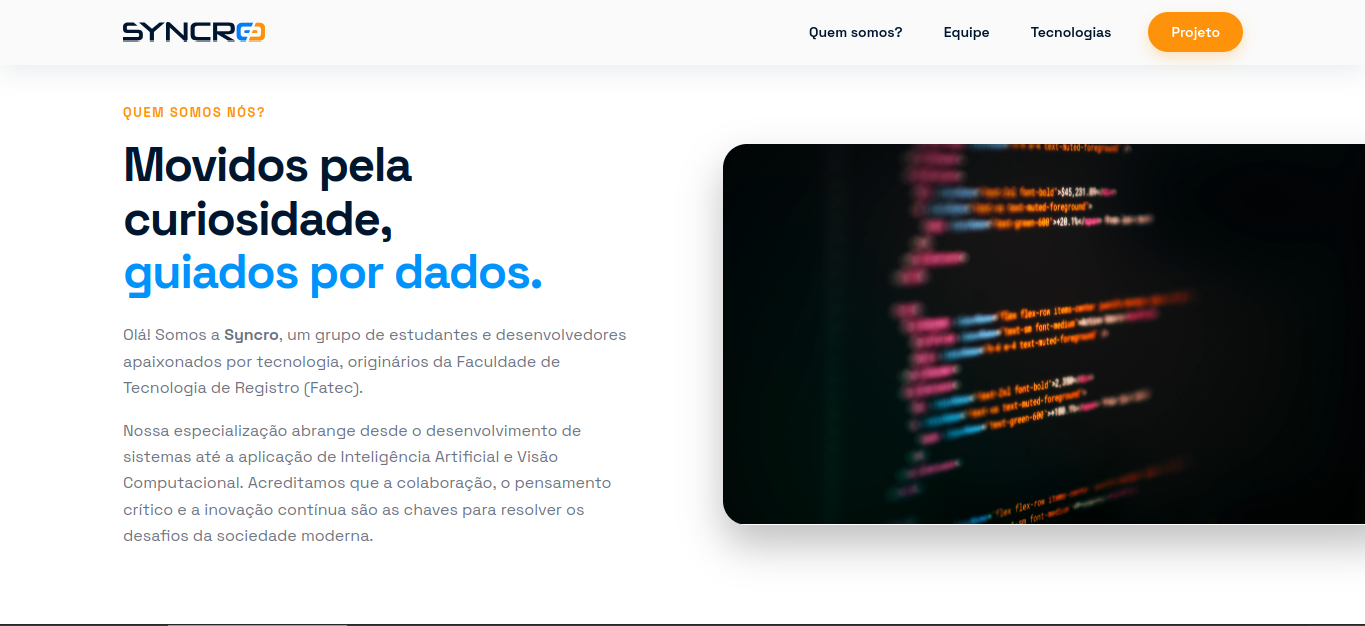
\includegraphics[width=\textwidth]{imgs/site_web/equipe/quemsomos.png}
\label{fig:website-quemsomos}
\end{figure}

\begin{figure}[H]
\centering
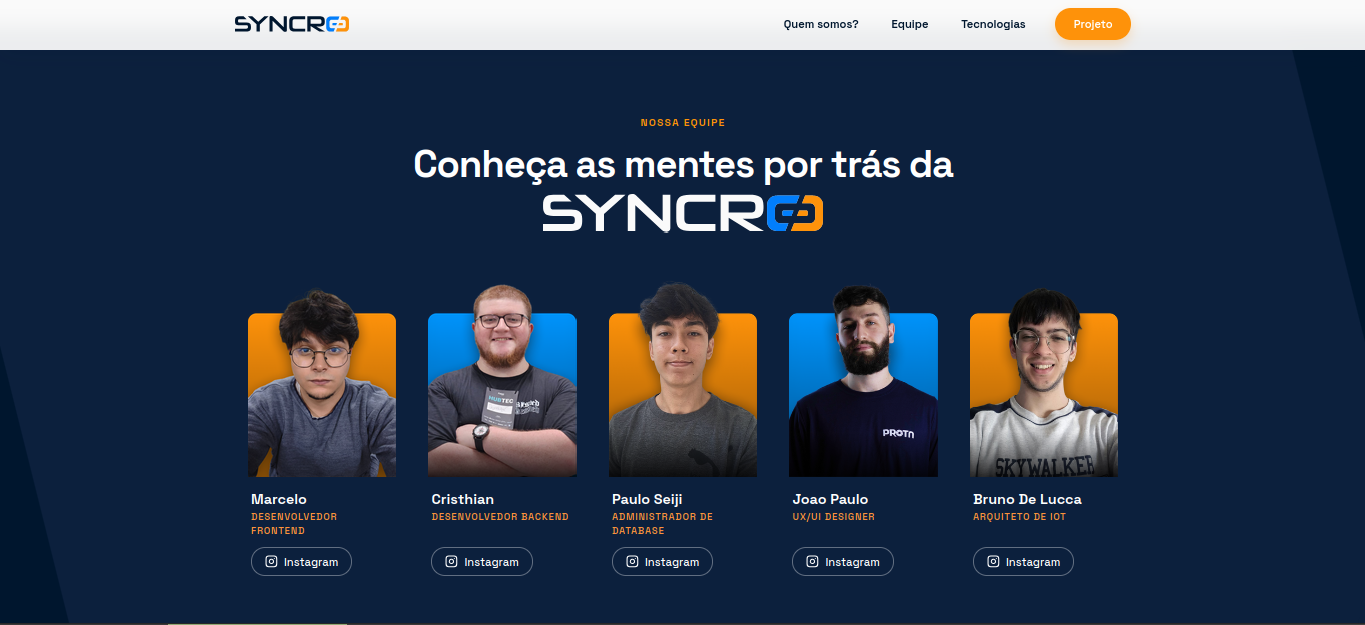
\includegraphics[width=\textwidth]{imgs/site_web/equipe/equipe.png}
\label{fig:website-equipe}
\end{figure}

\begin{figure}[H]
\centering
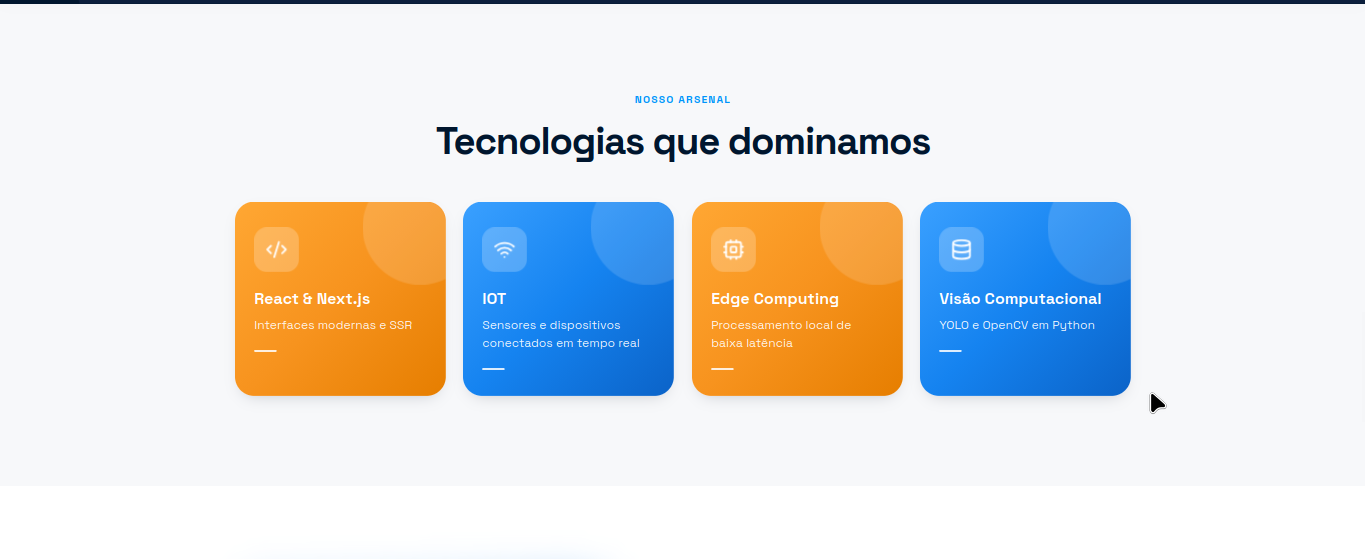
\includegraphics[width=\textwidth]{imgs/site_web/equipe/arsenal.png}
\label{fig:website-arsenal}
\end{figure}

\begin{figure}[H]
\centering
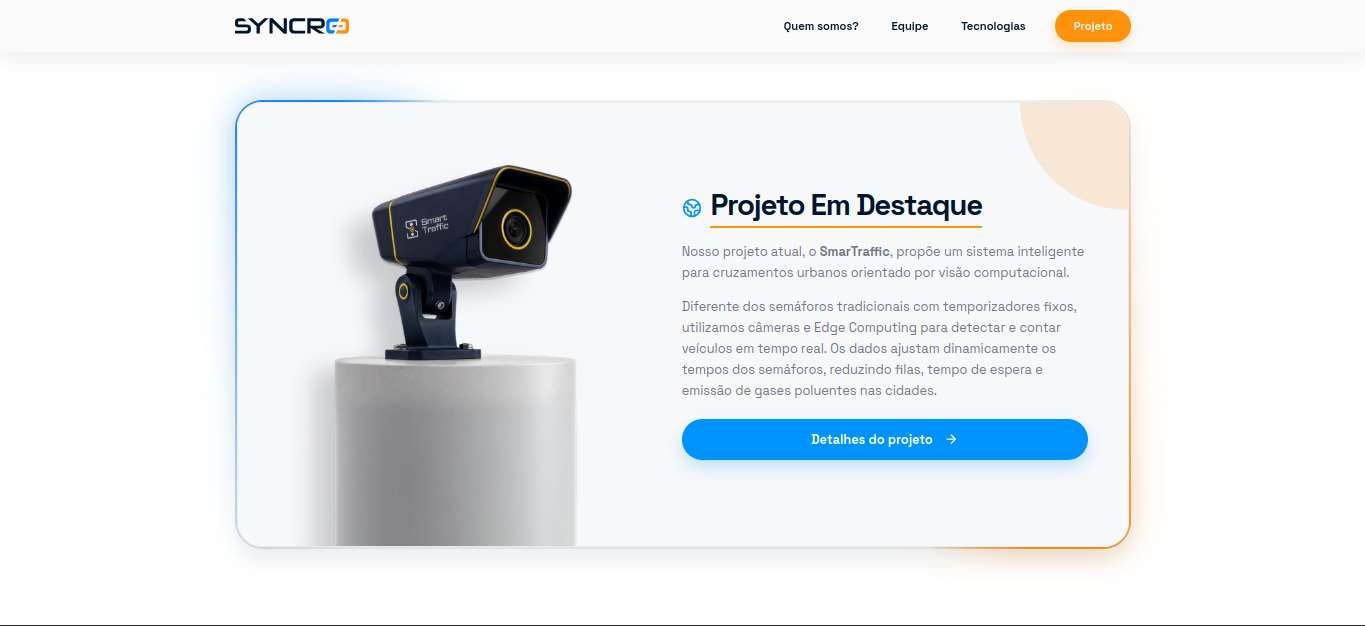
\includegraphics[width=\textwidth]{imgs/site_web/equipe/projetoemdestaque.png}
\label{fig:website-projetoemdestaque}
\end{figure}

\begin{figure}[H]
\centering
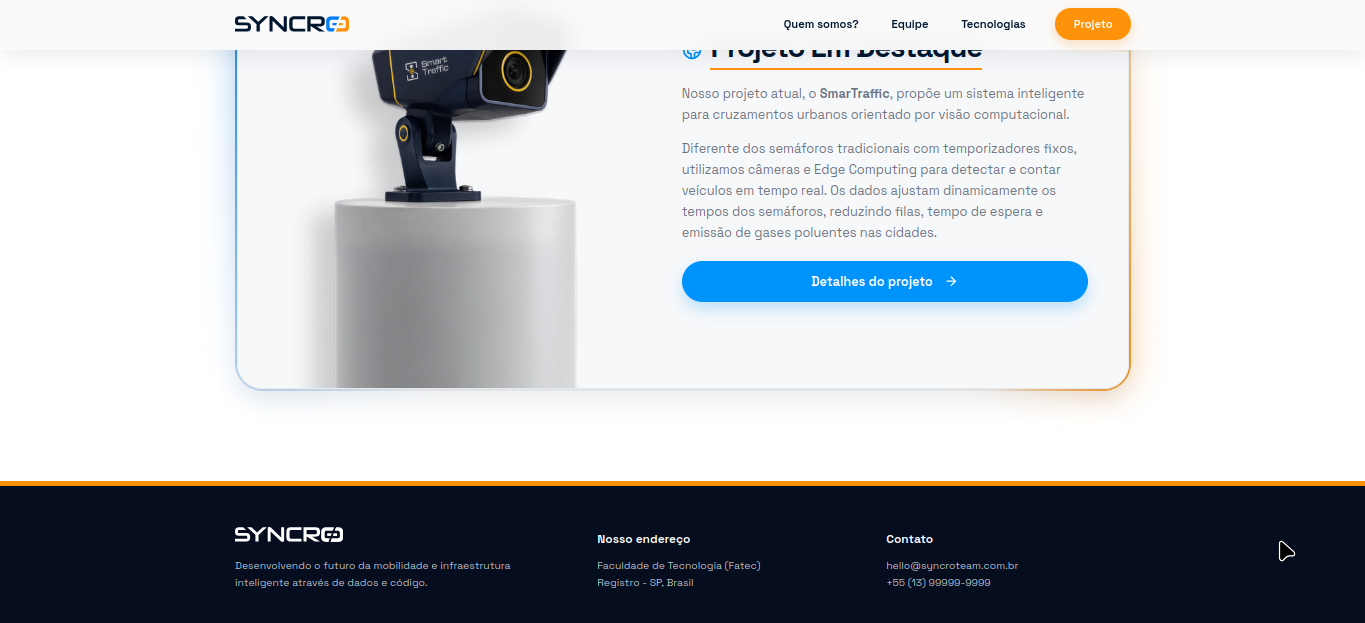
\includegraphics[width=\textwidth]{imgs/site_web/equipe/footer.png}
\caption{Página inicial do website da equipe}
\label{fig:website-footer}
\end{figure}

\subsection{Mapa do Site do Projeto}

O mapa do site (sitemap) mostra a hierarquia e organização das páginas do website do projeto:

\begin{figure}[H]
\centering
\begin{tikzpicture}[
    level 1/.style={sibling distance=4cm, level distance=1.5cm},
    level 2/.style={sibling distance=2cm, level distance=1.5cm},
    every node/.style={rectangle, draw, rounded corners, 
                       fill=secondarycolor!20, 
                       text width=2.5cm, 
                       align=center,
                       font=\small}
]
\node {SmarTraffic}
    child {node {Inicio/Home}
        child {node {Como funciona}}
        child {node {Tecnologias}}
        child {node {Protótipo}}
        child {node {Equipe}}
    }
    child {node {Projeto}
        child {node {Geral}}
        child {node {Escopo}}
    }
    child {node {Documentacao}
        child {node {Fluxo}}
        child {node {Componentes}}
    };
\end{tikzpicture}
\caption{Estrutura de navegação do website do projeto}
\label{fig:sitemap-projeto}
\end{figure}

\subsection{Screenshots do Website do Projeto}

\begin{figure}[H]
\centering
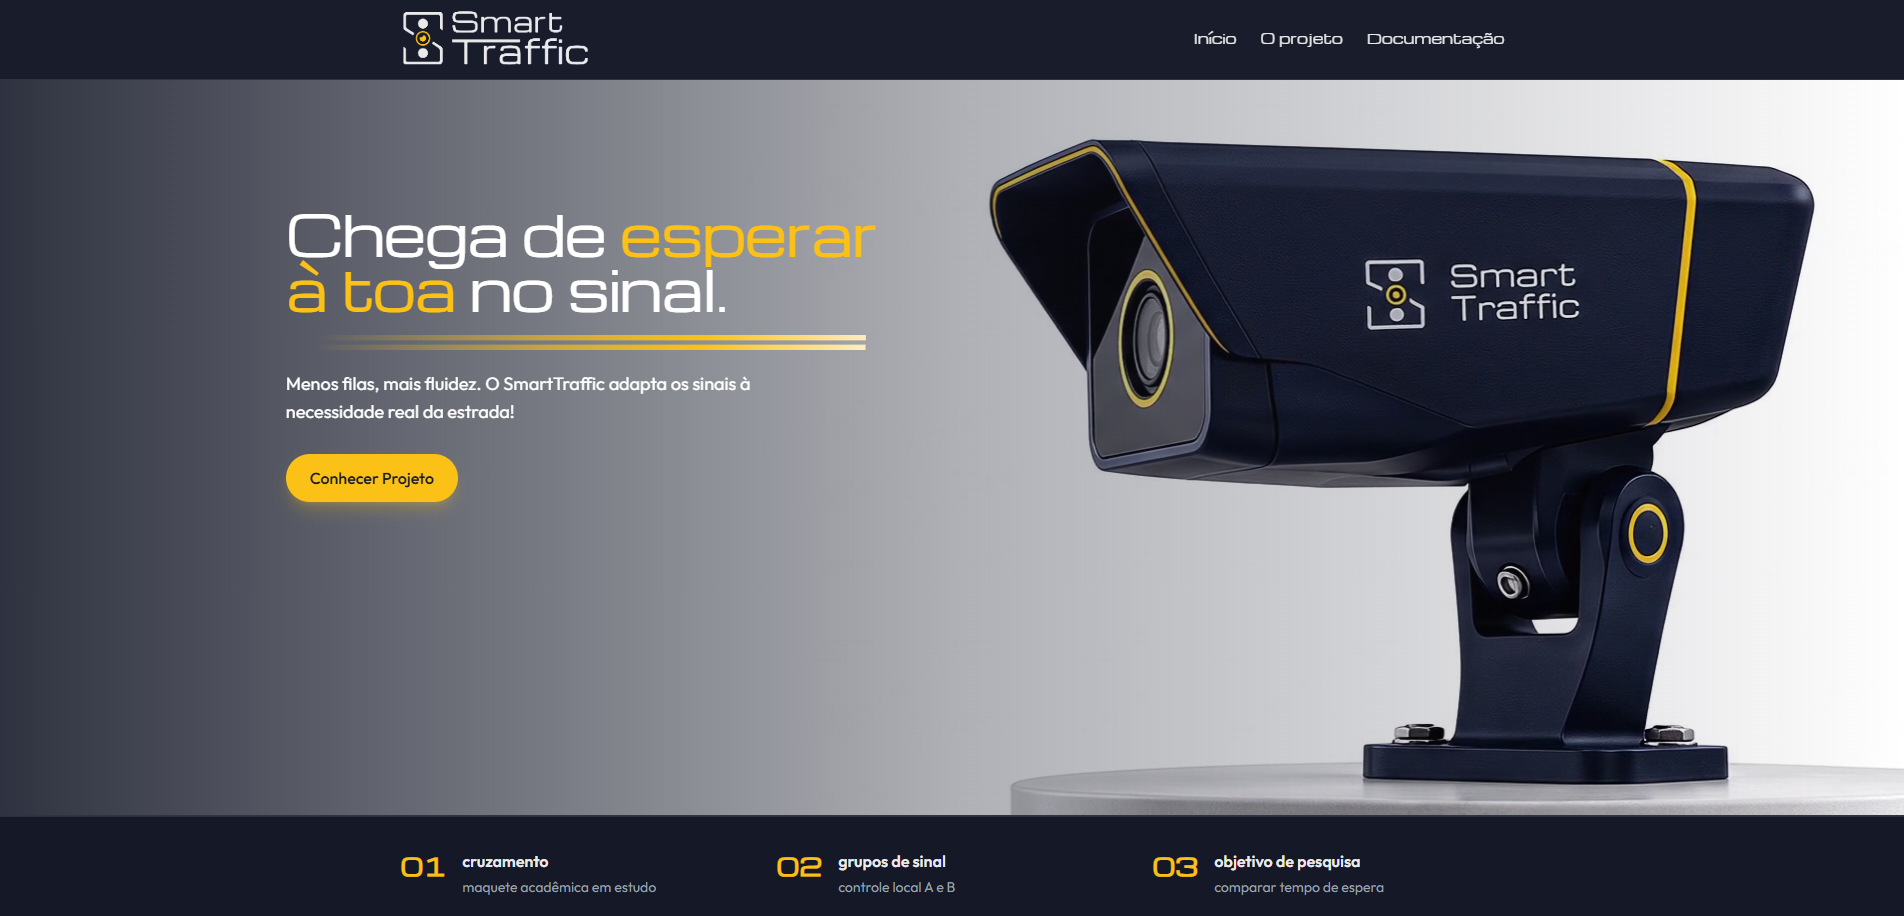
\includegraphics[width=\textwidth]{imgs/site_web/projeto/website_projeto_header.png}
\caption{Cabeçalho do website do projeto}
\label{fig:web-header}
\end{figure}

\begin{figure}[H]
\centering
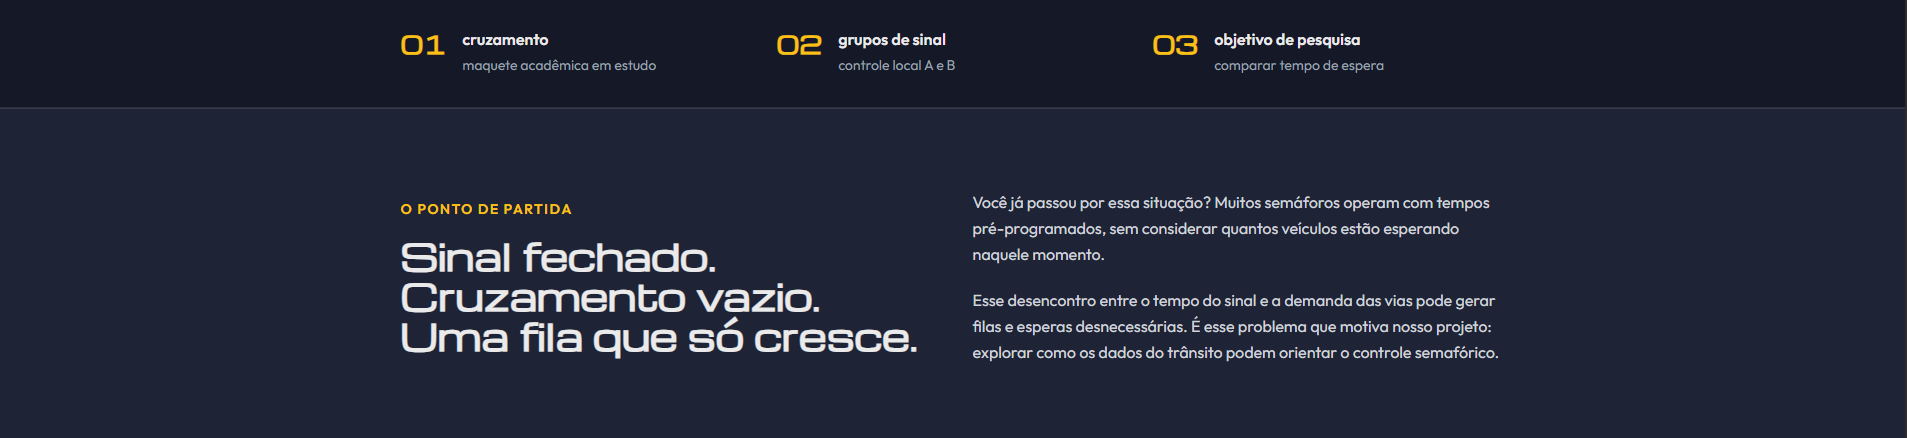
\includegraphics[width=\textwidth]{imgs/site_web/projeto/website_projeto_homepage2.png}
\caption{Página inicial do website do projeto (2)}
\label{fig:web-home-2}
\end{figure}

\begin{figure}[H]
\centering
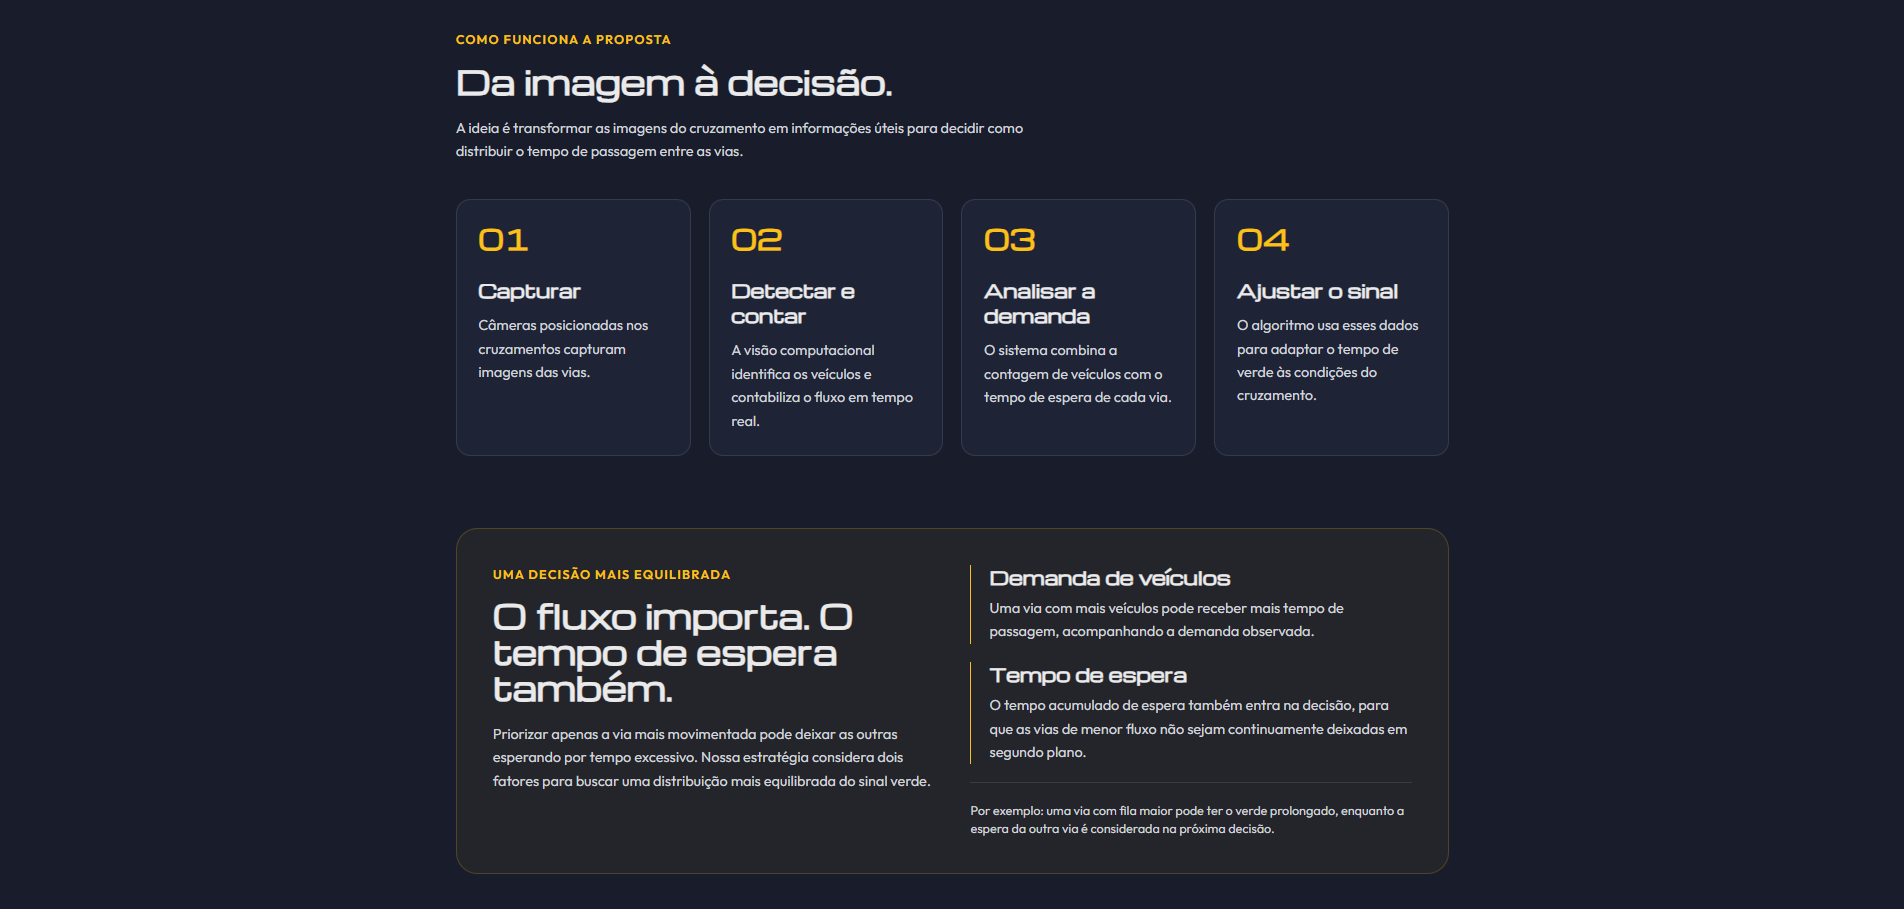
\includegraphics[width=\textwidth]{imgs/site_web/projeto/website_projeto_homepage3.png}
\caption{Página inicial do website do projeto (3)}
\label{fig:web-home-3}
\end{figure}

\begin{figure}[H]
\centering
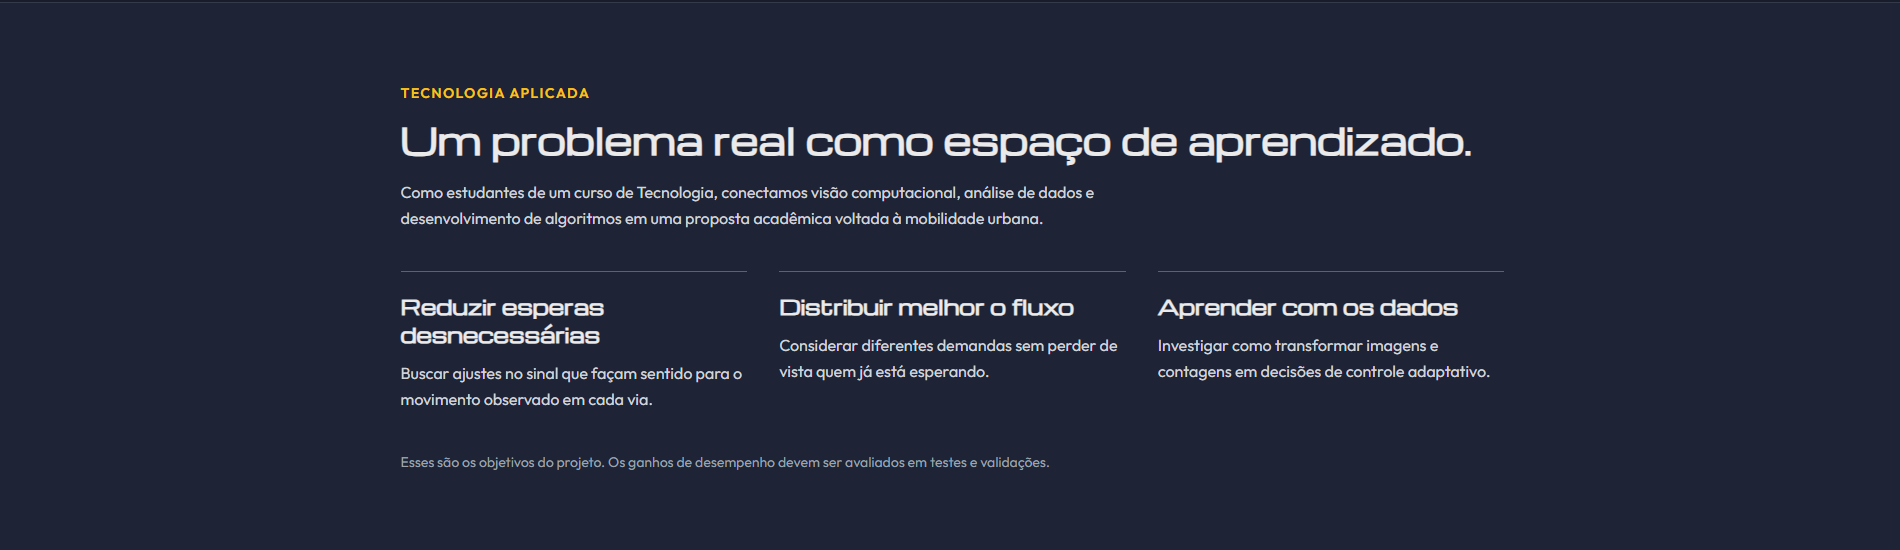
\includegraphics[width=\textwidth]{imgs/site_web/projeto/website_projeto_homepage4.png}
\caption{Página inicial do website do projeto (4)}
\label{fig:web-home-4}
\end{figure}

\begin{figure}[H]
\centering
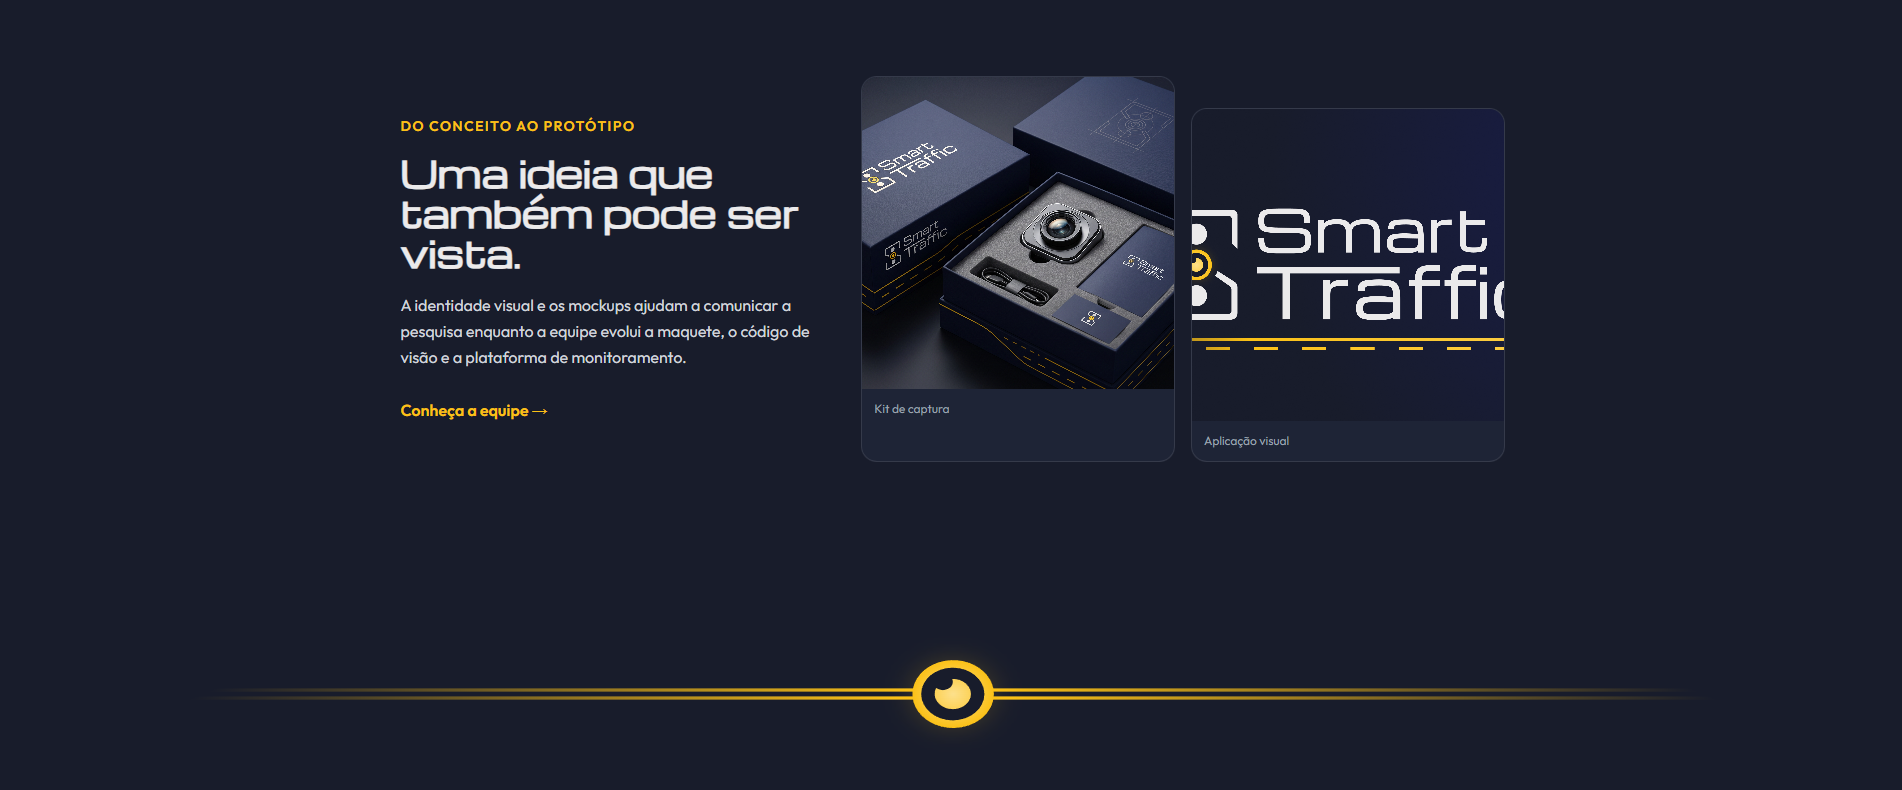
\includegraphics[width=\textwidth]{imgs/site_web/projeto/website_projeto_homepage5.png}
\caption{Página inicial do website do projeto (5)}
\label{fig:web-home-5}
\end{figure}

\begin{figure}[H]
\centering
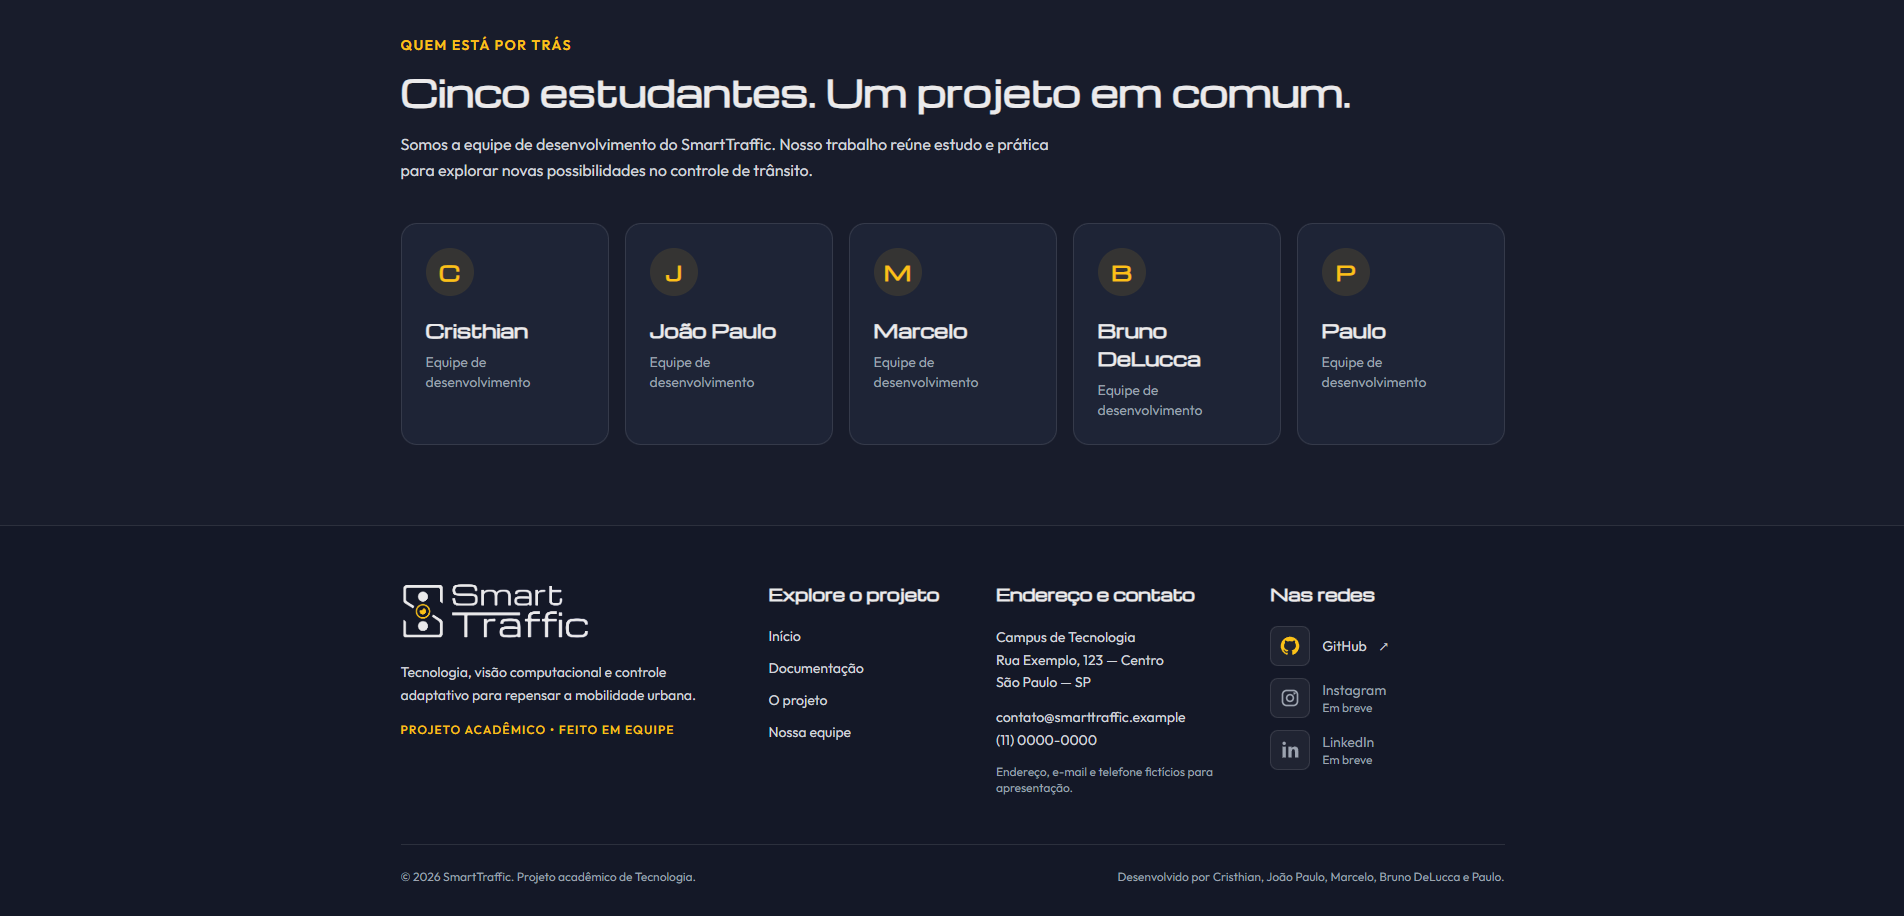
\includegraphics[width=\textwidth]{imgs/site_web/projeto/website_projeto_homepagefooter.png}
\caption{Página inicial do website do projeto (rodapé)}
\label{fig:web-home-footer}
\end{figure}

\begin{figure}[H]
\centering
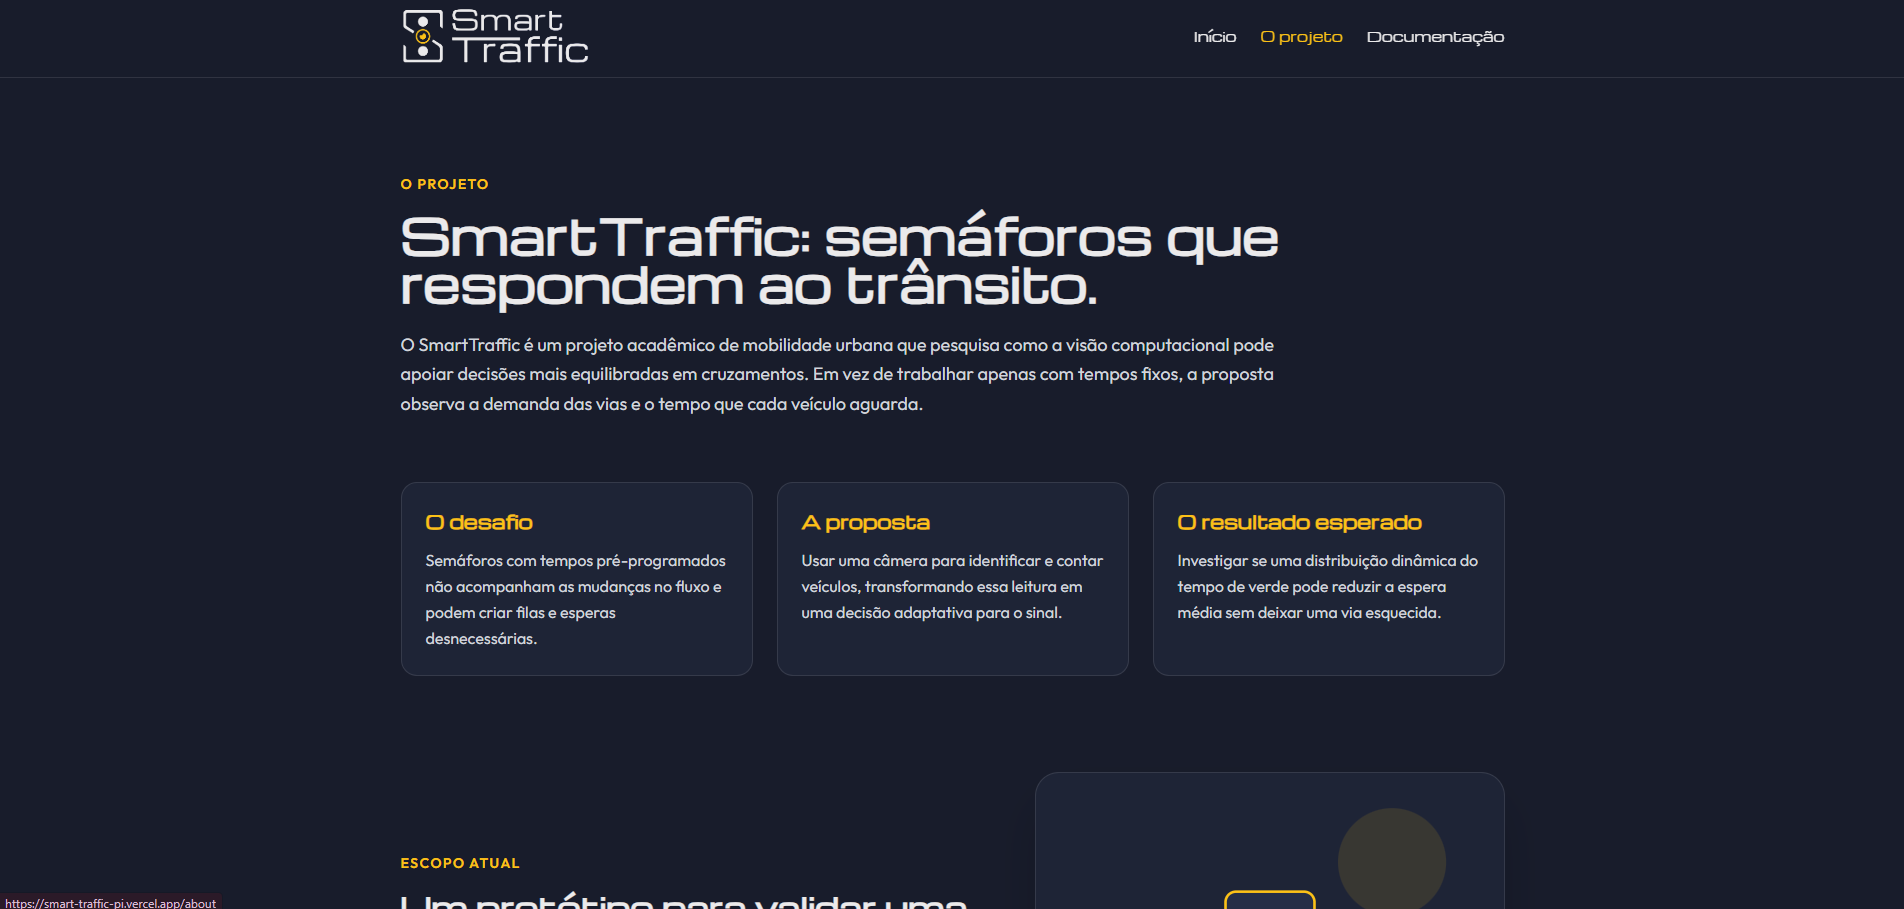
\includegraphics[width=\textwidth]{imgs/site_web/projeto/website_projeto_projeto1.png}
\caption{Página do projeto (1)}
\label{fig:web-projeto-1}
\end{figure}

\begin{figure}[H]
\centering
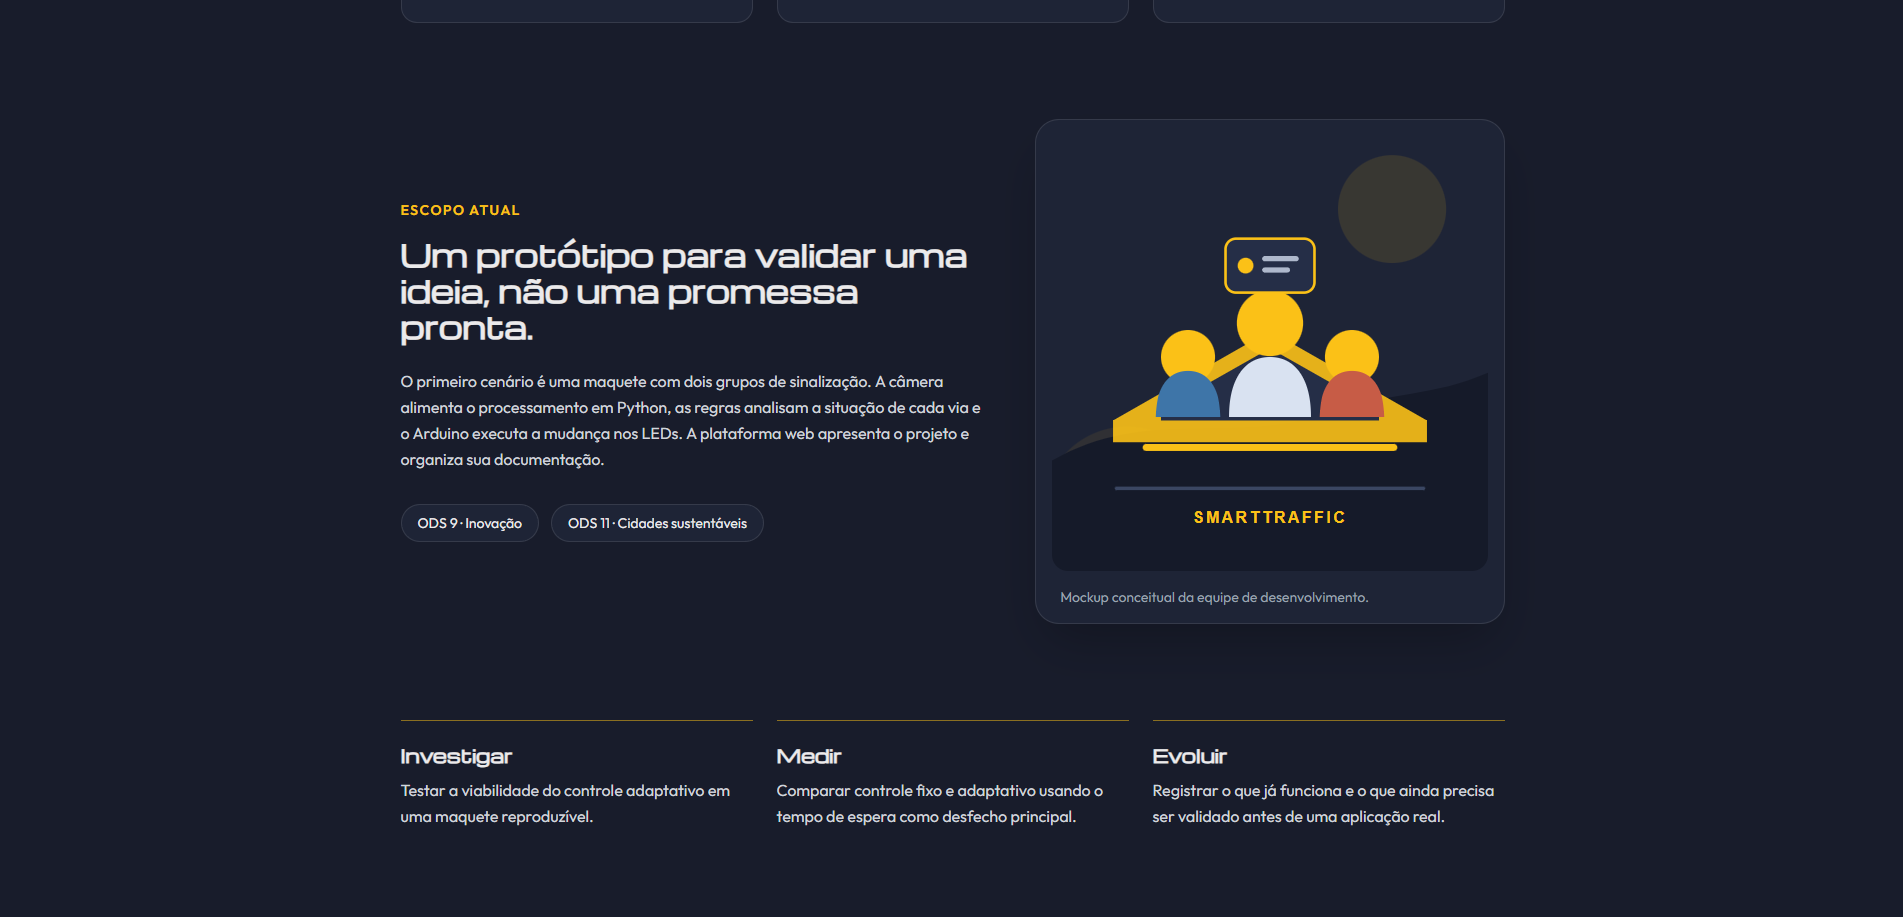
\includegraphics[width=\textwidth]{imgs/site_web/projeto/website_projeto_projeto2.png}
\caption{Página relacionada ao projeto (2)}
\label{fig:web-projeto-2}
\end{figure}

\begin{figure}[H]
\centering
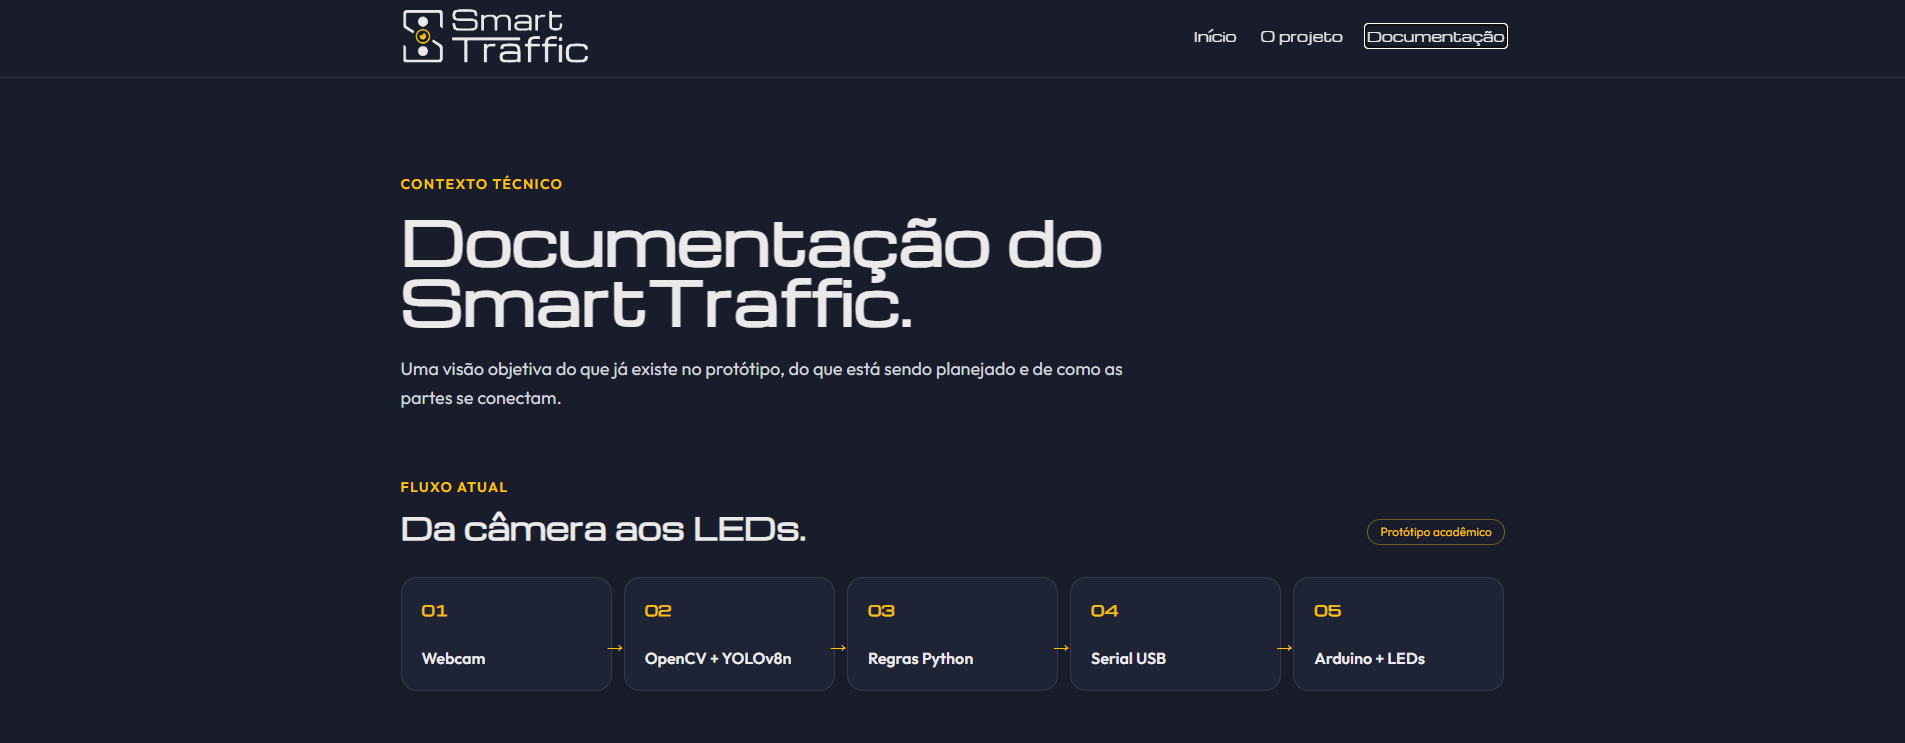
\includegraphics[width=\textwidth]{imgs/site_web/projeto/website_projeto_documentacao.png}
\caption{Página de documentação do projeto (1)}
\label{fig:web-doc-1}
\end{figure}

\begin{figure}[H]
\centering
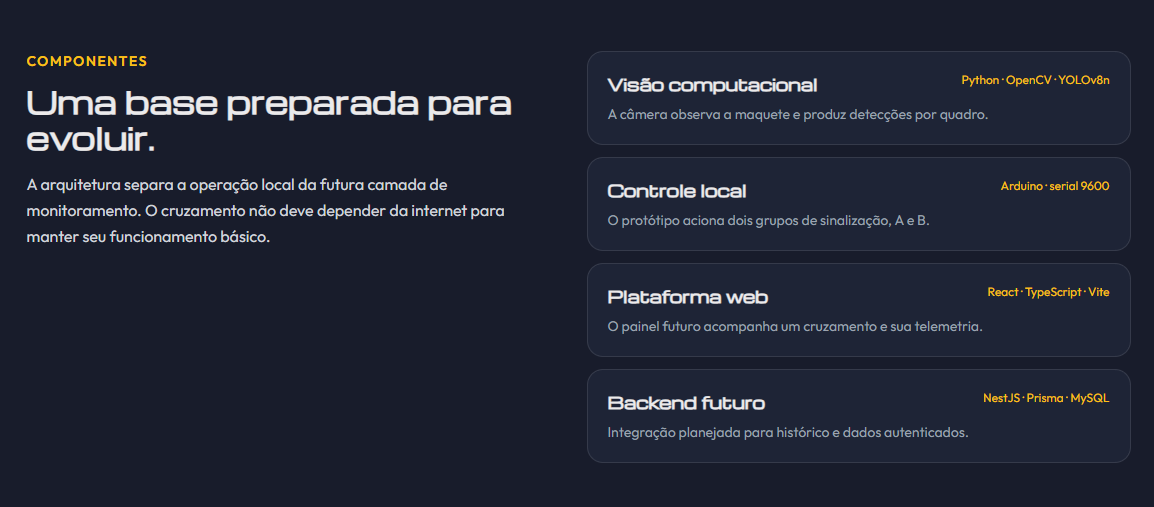
\includegraphics[width=\textwidth]{imgs/site_web/projeto/website_projeto_documentacao2.png}
\caption{Página de documentação do projeto (2)}
\label{fig:web-doc-2}
\end{figure}

\begin{figure}[H]
\centering
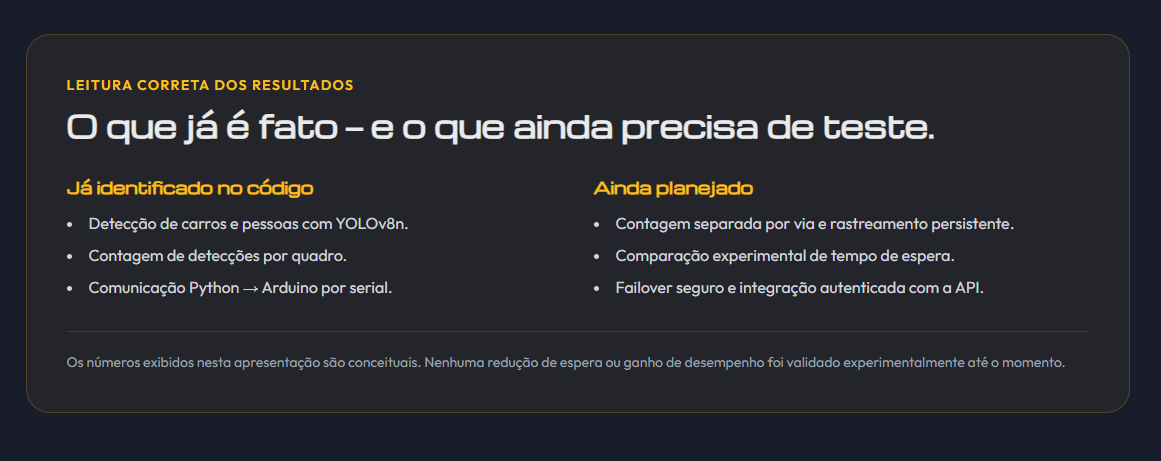
\includegraphics[width=\textwidth]{imgs/site_web/projeto/website_projeto_documentacao3.png}
\caption{Página relacionada à documentação do projeto (3)}
\label{fig:web-doc-3}
\end{figure}

\subsection{Telas Técnicas do Projeto}

\begin{table}[H]
\centering
\caption{Stack Tecnológicas}
\label{tab:stack-web}
\begin{tabular}{|l|l|p{5cm}|}
\hline
\textbf{Camada} & \textbf{Tecnologia} & \textbf{Descrição} \\
\hline
Plataforma Web & React, TypeScript & Biblioteca JavaScript para interfaces \\
Controle Local/Dispositivo Físico & Arduino, C++ & Kit para utilização de equipamentos físicos \\
Hospedagem & Vercel & Deploy e hosting gratuito \\
Visão Computacional & Python, OpenCV e YOLOv8n & Rede Neural para detecção de veículos e pedestres \\
Backend & Nest.js, Prisma, MySQL & Toda lógica de negócio do projeto \\
\hline
\end{tabular}
\end{table}

% ===== DIAGRAMAS UML =====
\section{Diagramas UML: Modelagem Visual do Sistema}

A Unified Modeling Language (UML) \cite{kumar2024} é uma linguagem de modelagem visual usada para especificar, visualizar, construir e documentar artefatos de sistemas de software.\footnote{A UML foi padronizada pela Object Management Group (OMG) em 1997.}

\subsection{Diagrama de Casos de Uso}

O diagrama de casos de uso representa as funcionalidades do sistema do ponto de vista do usuário:

\begin{figure}[H]
\centering
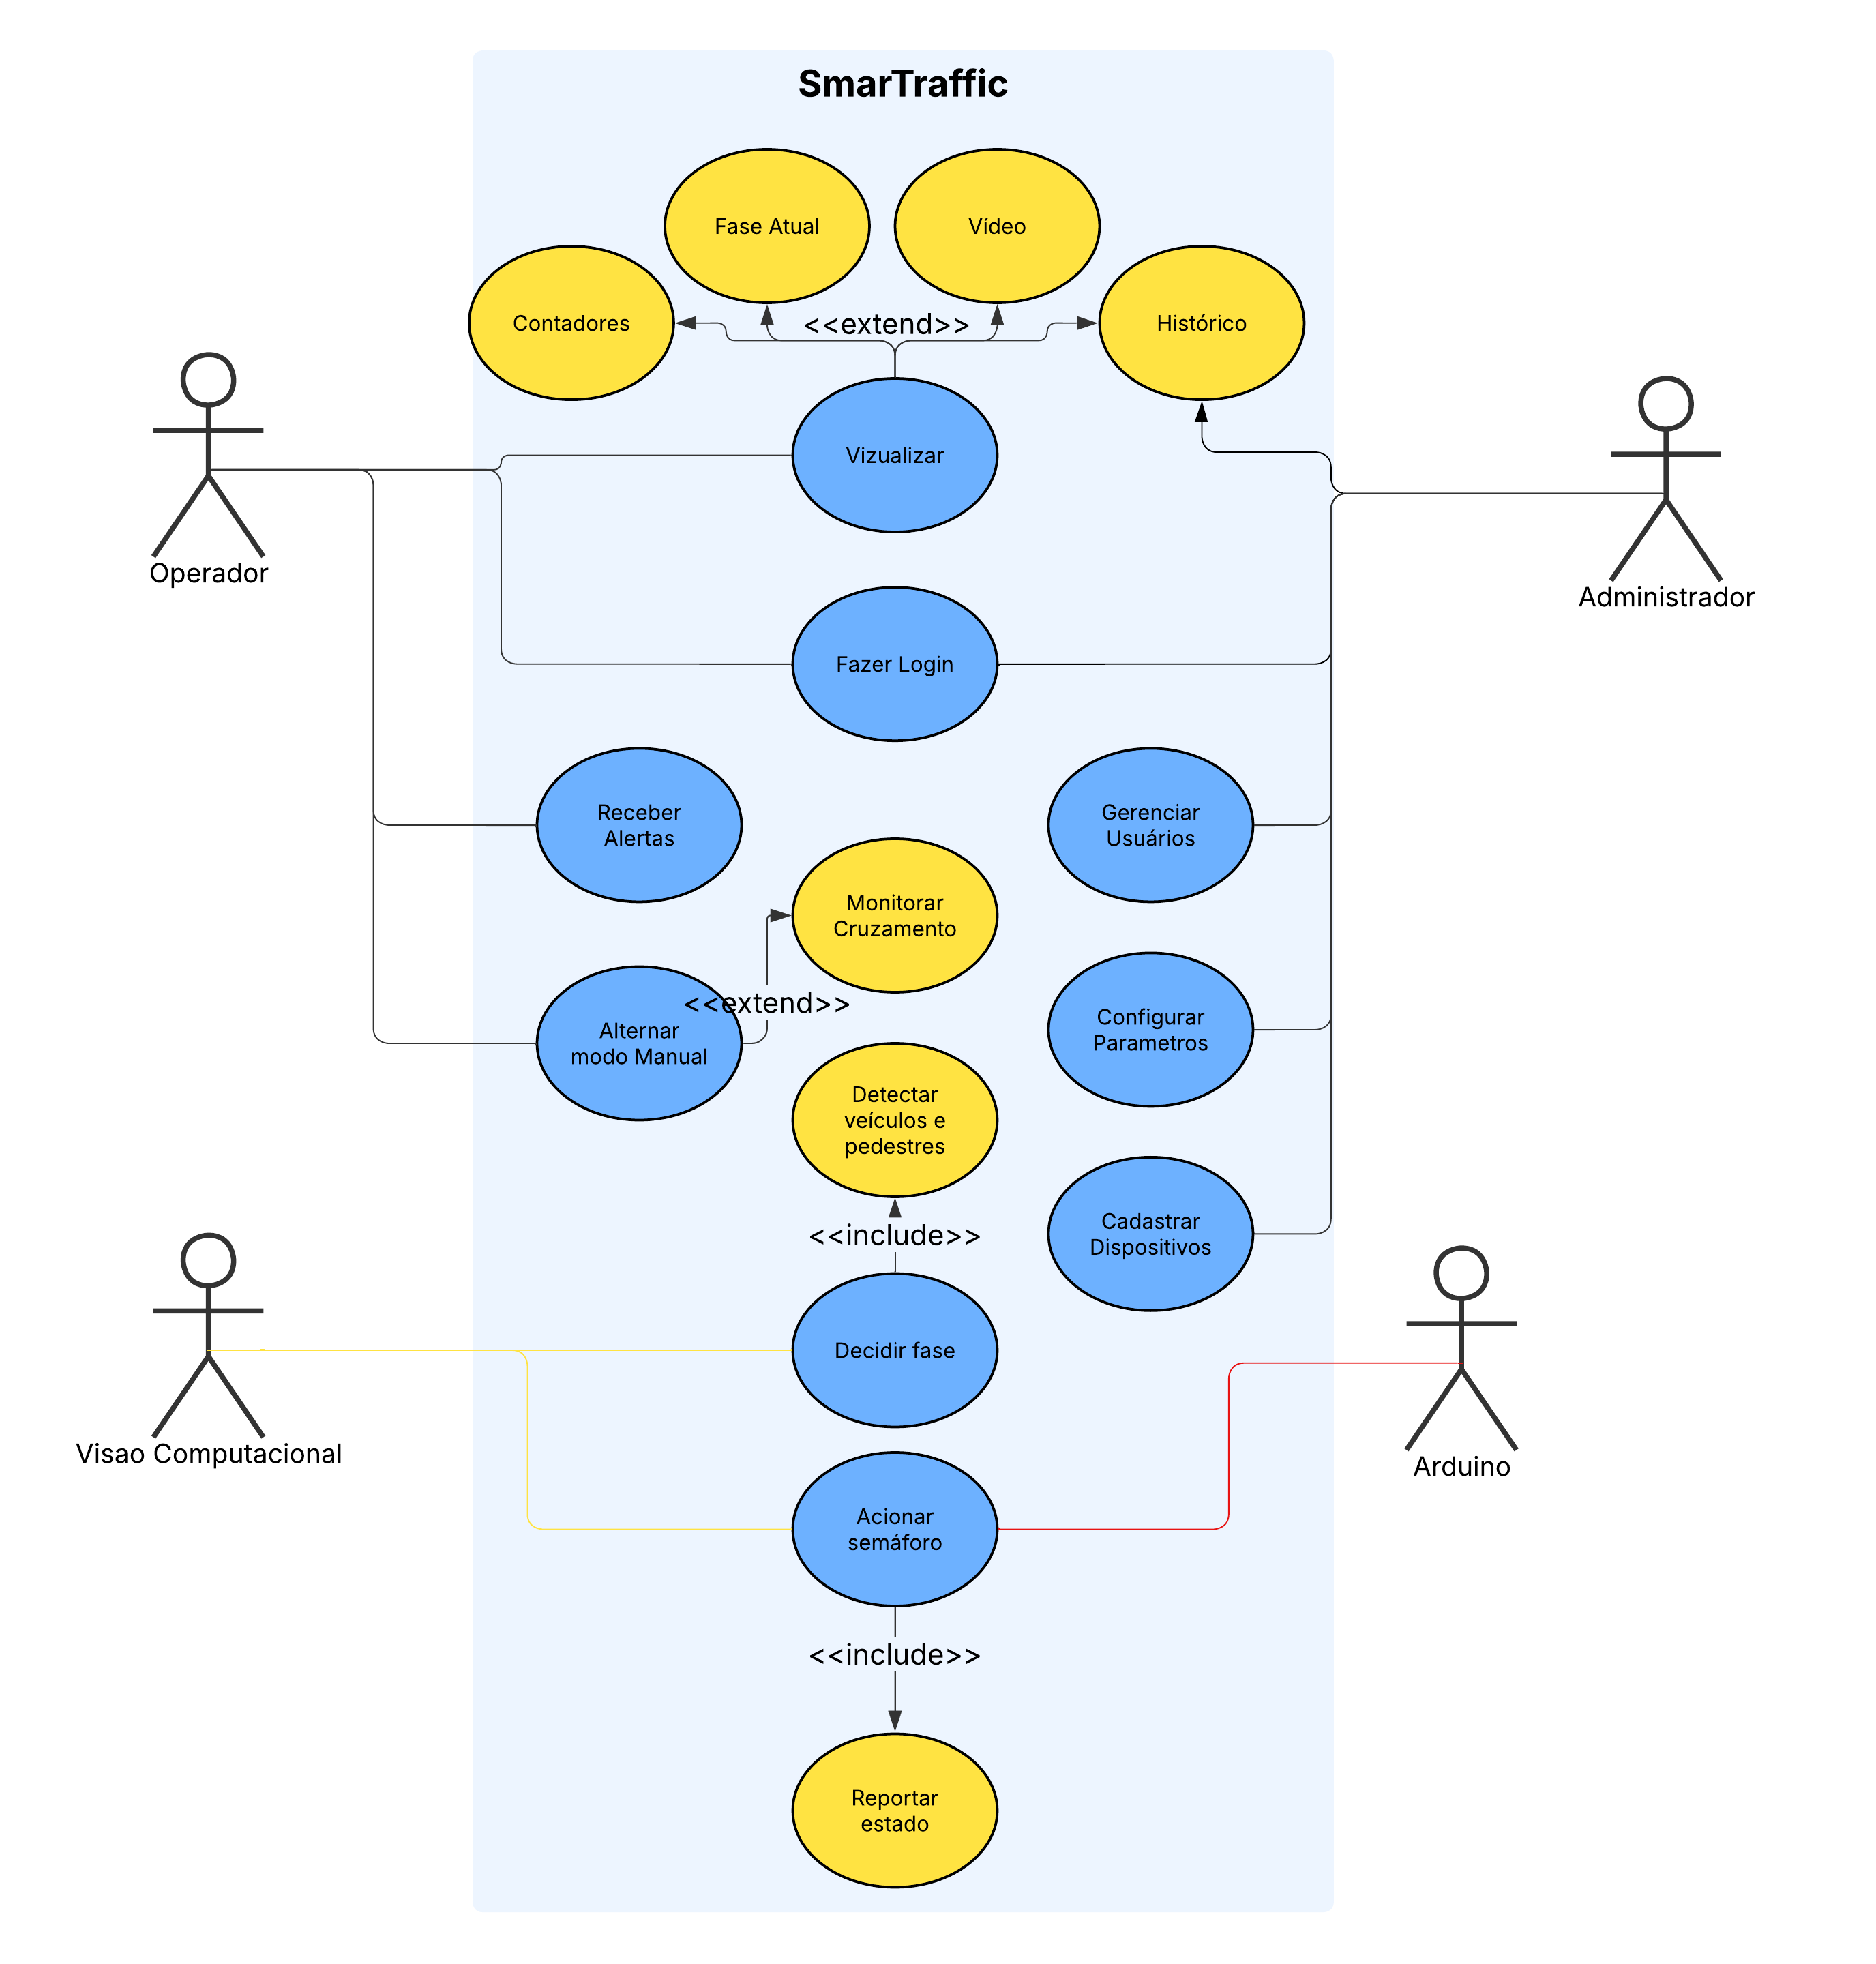
\includegraphics[width=\textwidth]{imgs/simple-use-case-diagram.png}
\caption{Diagrama de Caso de Uso do SmarTraffic}
\label{fig:use-case-diagram}
\end{figure}

\subsection{Diagrama de Classes}

O diagrama de classes mostra a estrutura estática do sistema:

\begin{figure}[H]
\centering
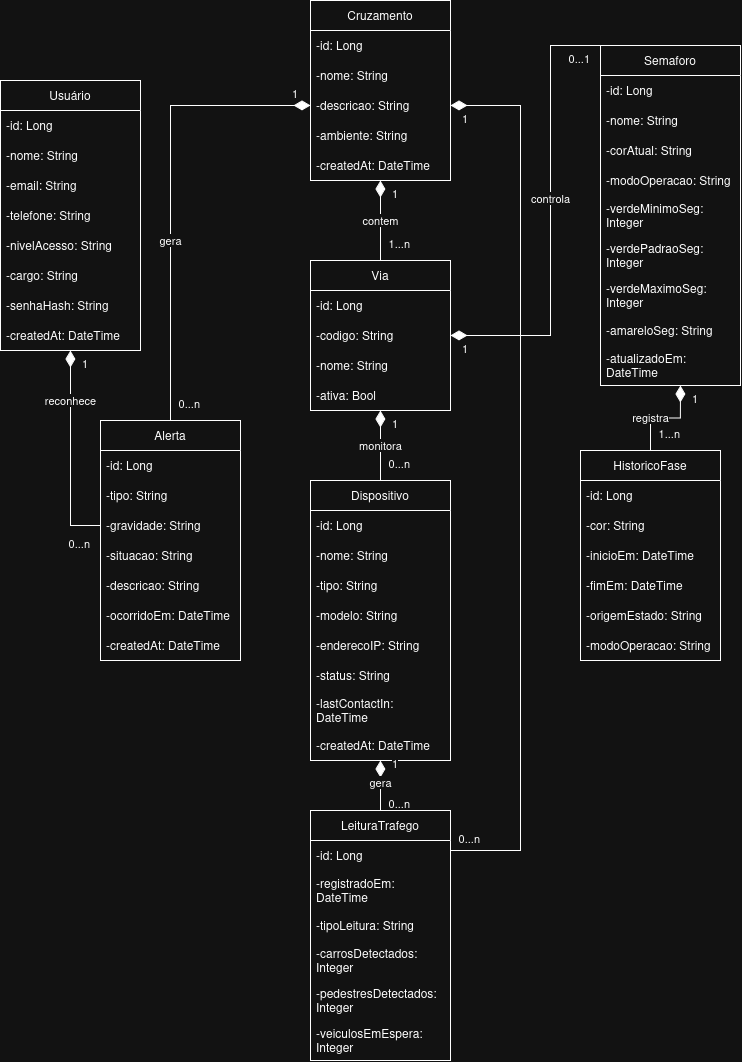
\includegraphics[width=\textwidth]{imgs/untitled-diagram.png}
\caption{Diagrama de Classes do Sistema}
\label{fig:class-diagram}
\end{figure}

\subsection{Diagrama de Objetos}

O diagrama de objetos mostra a estrutura estática do sistema utilizando dados fictícios:

\begin{figure}[H]
\centering
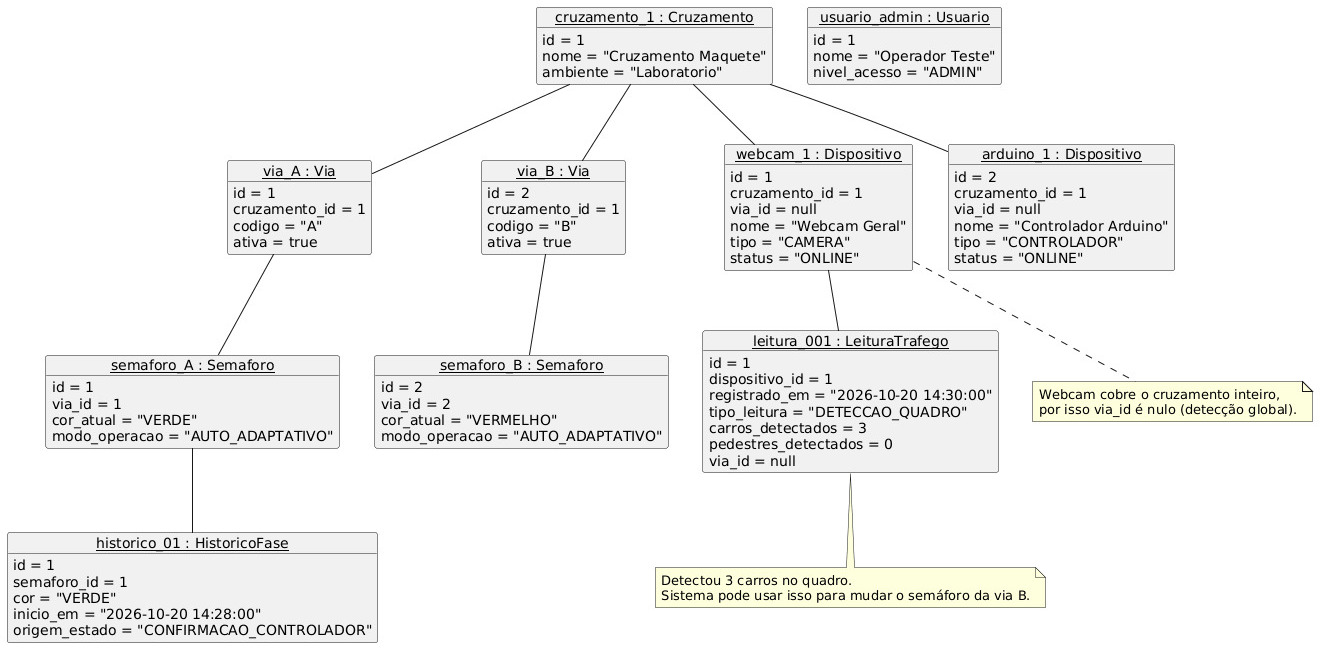
\includegraphics[width=\textwidth]{imgs/diagrama-de-objeto.jpeg}
\caption{Diagrama de Objetos do Sistema}
\label{fig:class-diagram}
\end{figure}

\subsubsection{Diagrama de Infraestrutura}

Para ilustrar como os componentes se conectam:

\begin{figure}[H]
\centering
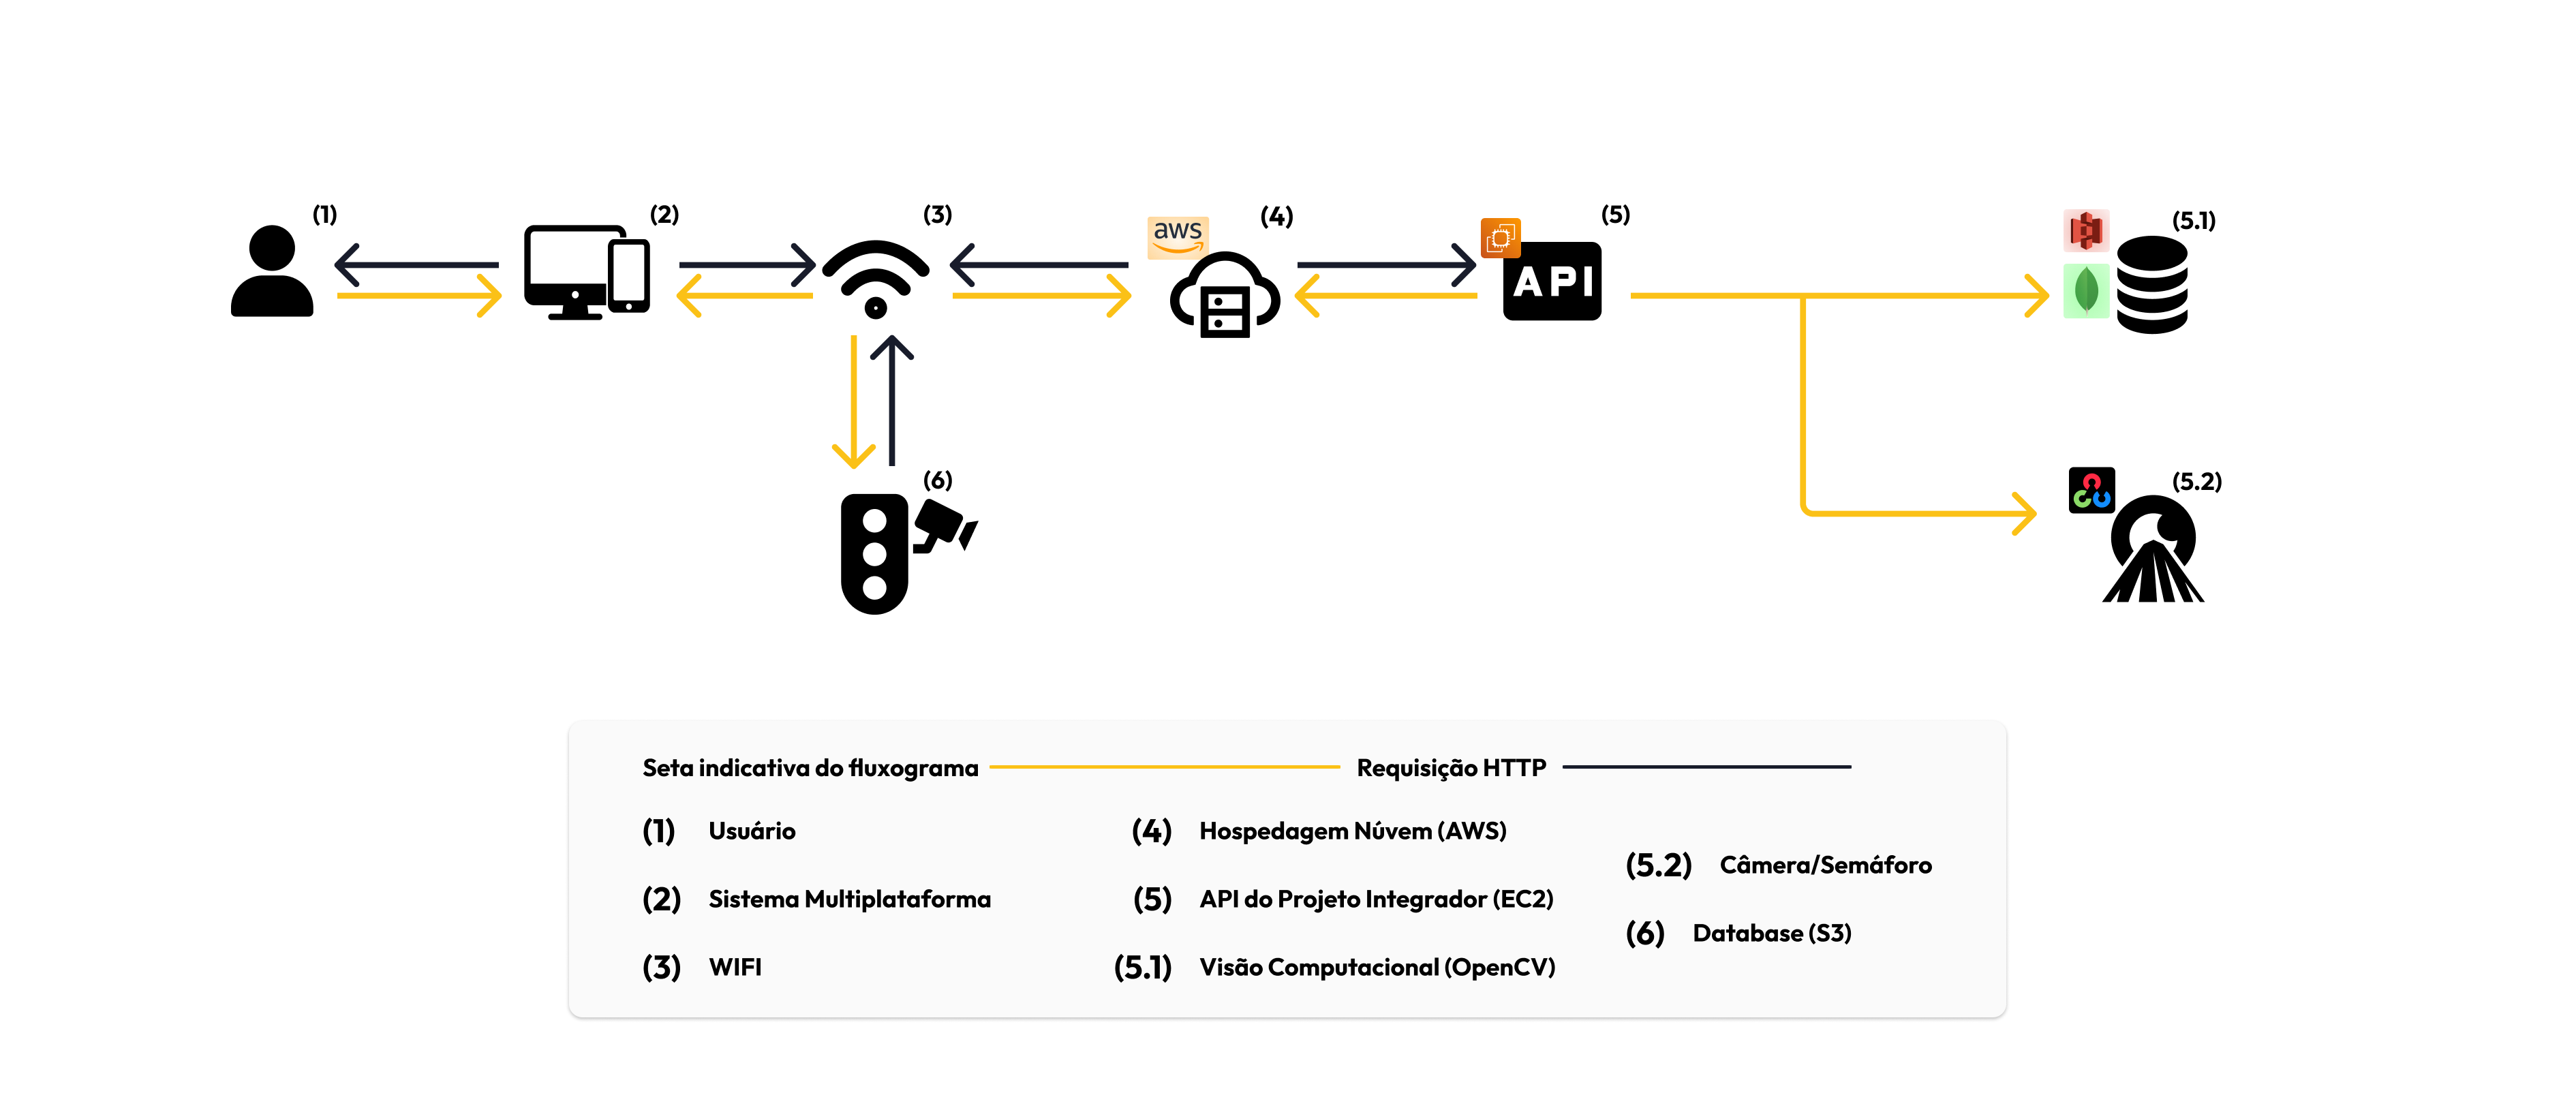
\includegraphics[width=\textwidth]{imgs/diagrama-de-rede-v1.png}
\caption{Diagrama de Infraestrutura do Sistema -- V1}
\label{fig:infra-v1}
\end{figure}

\begin{figure}[H]
\centering
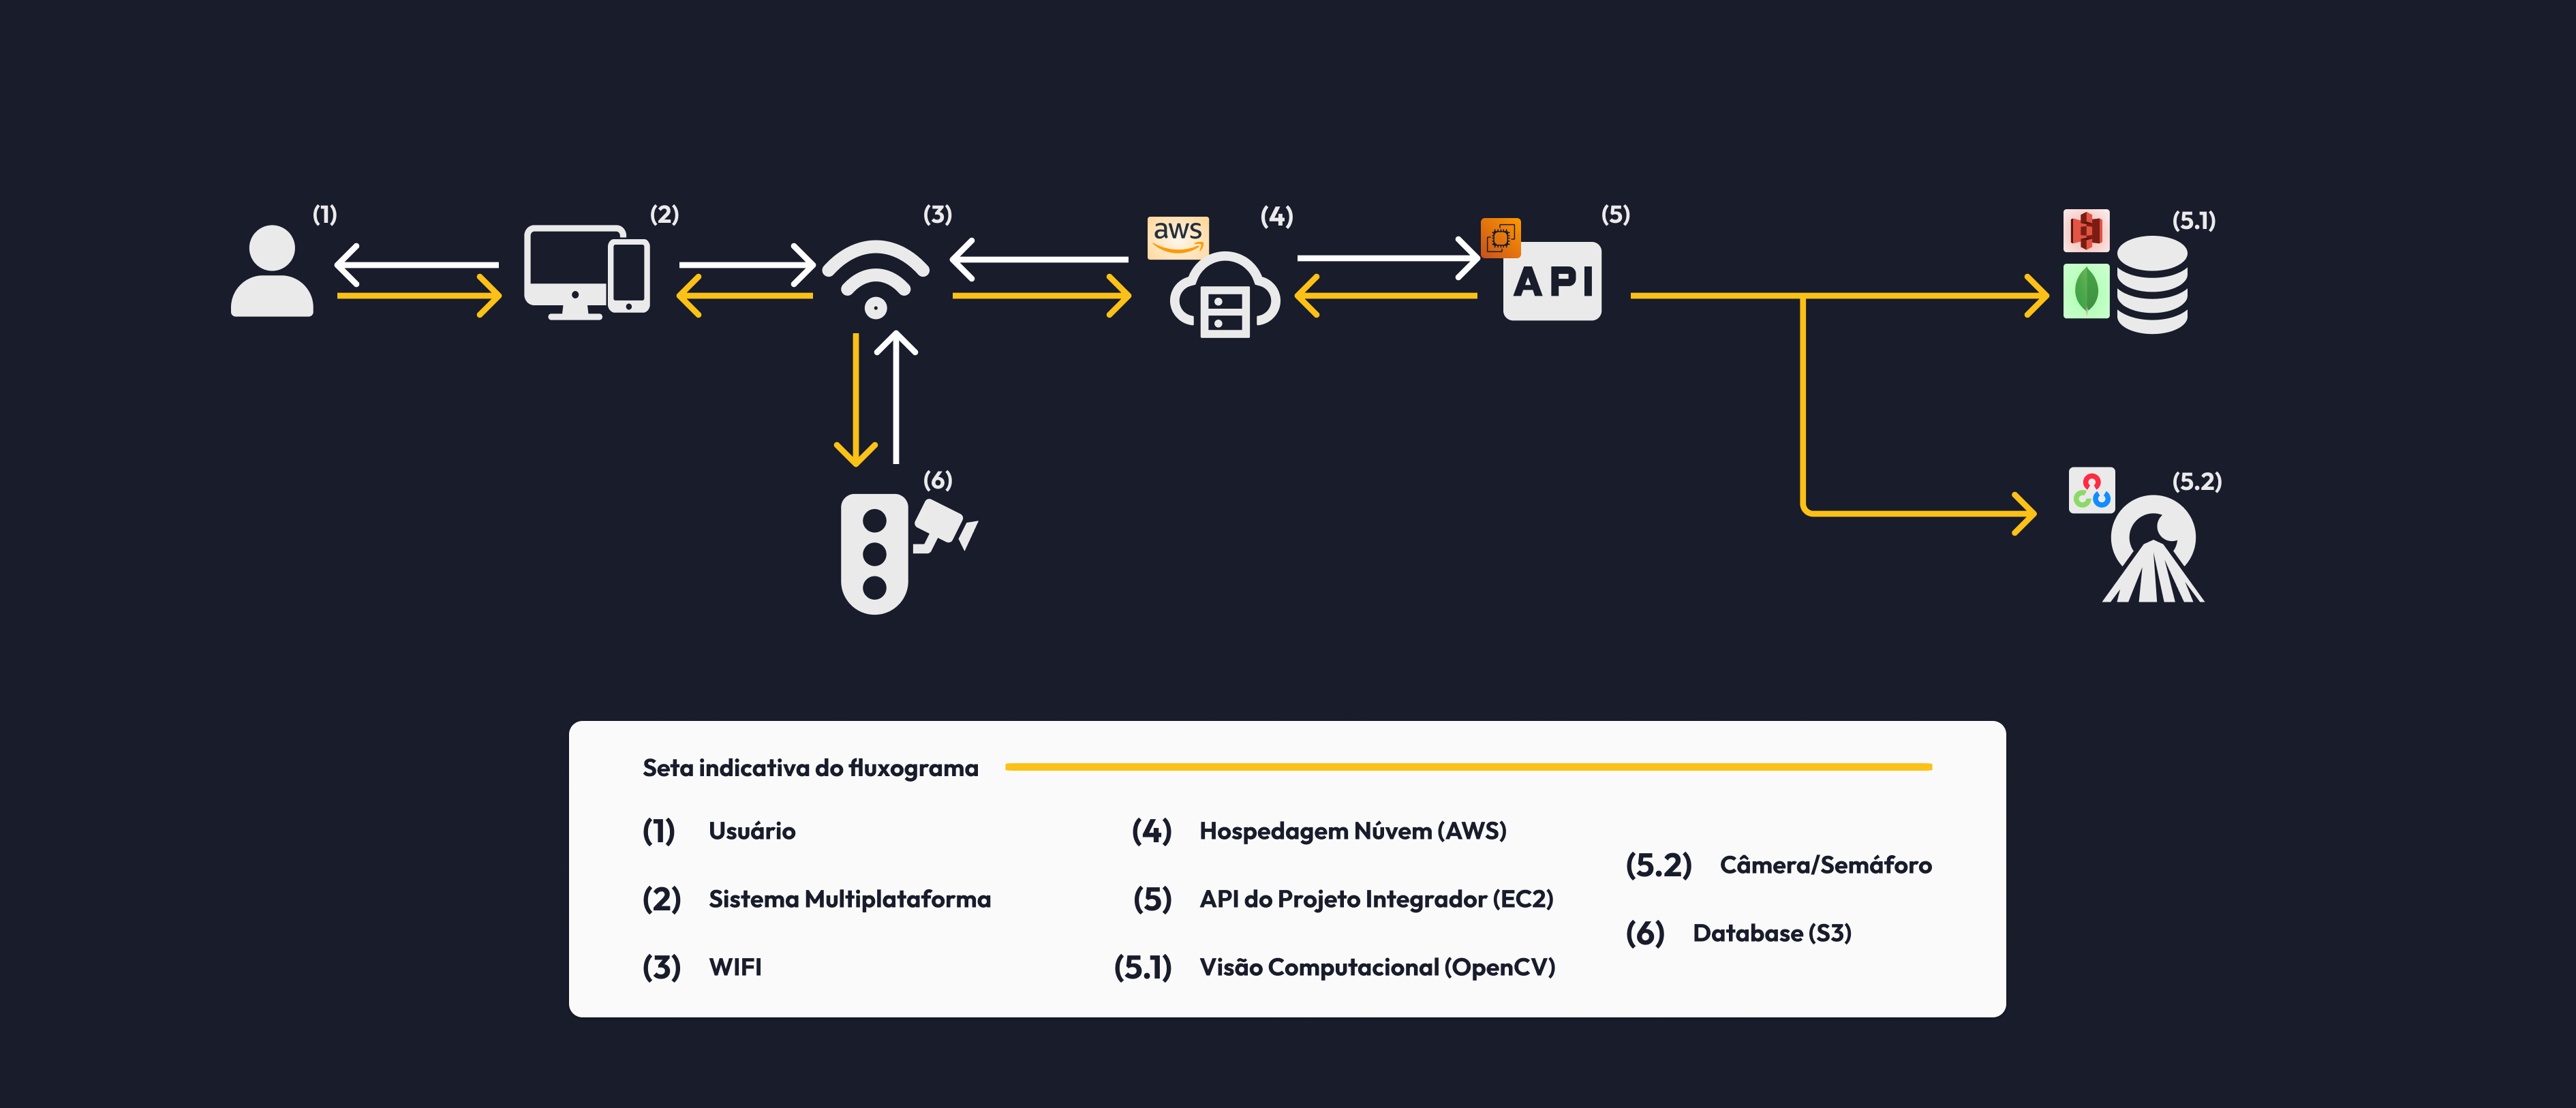
\includegraphics[width=\textwidth]{imgs/diagrama-de-rede-v2.png}
\caption{Diagrama de Infraestrutura do Sistema -- V2}
\label{fig:infra-v2}
\end{figure}

\begin{figure}[H]
\centering
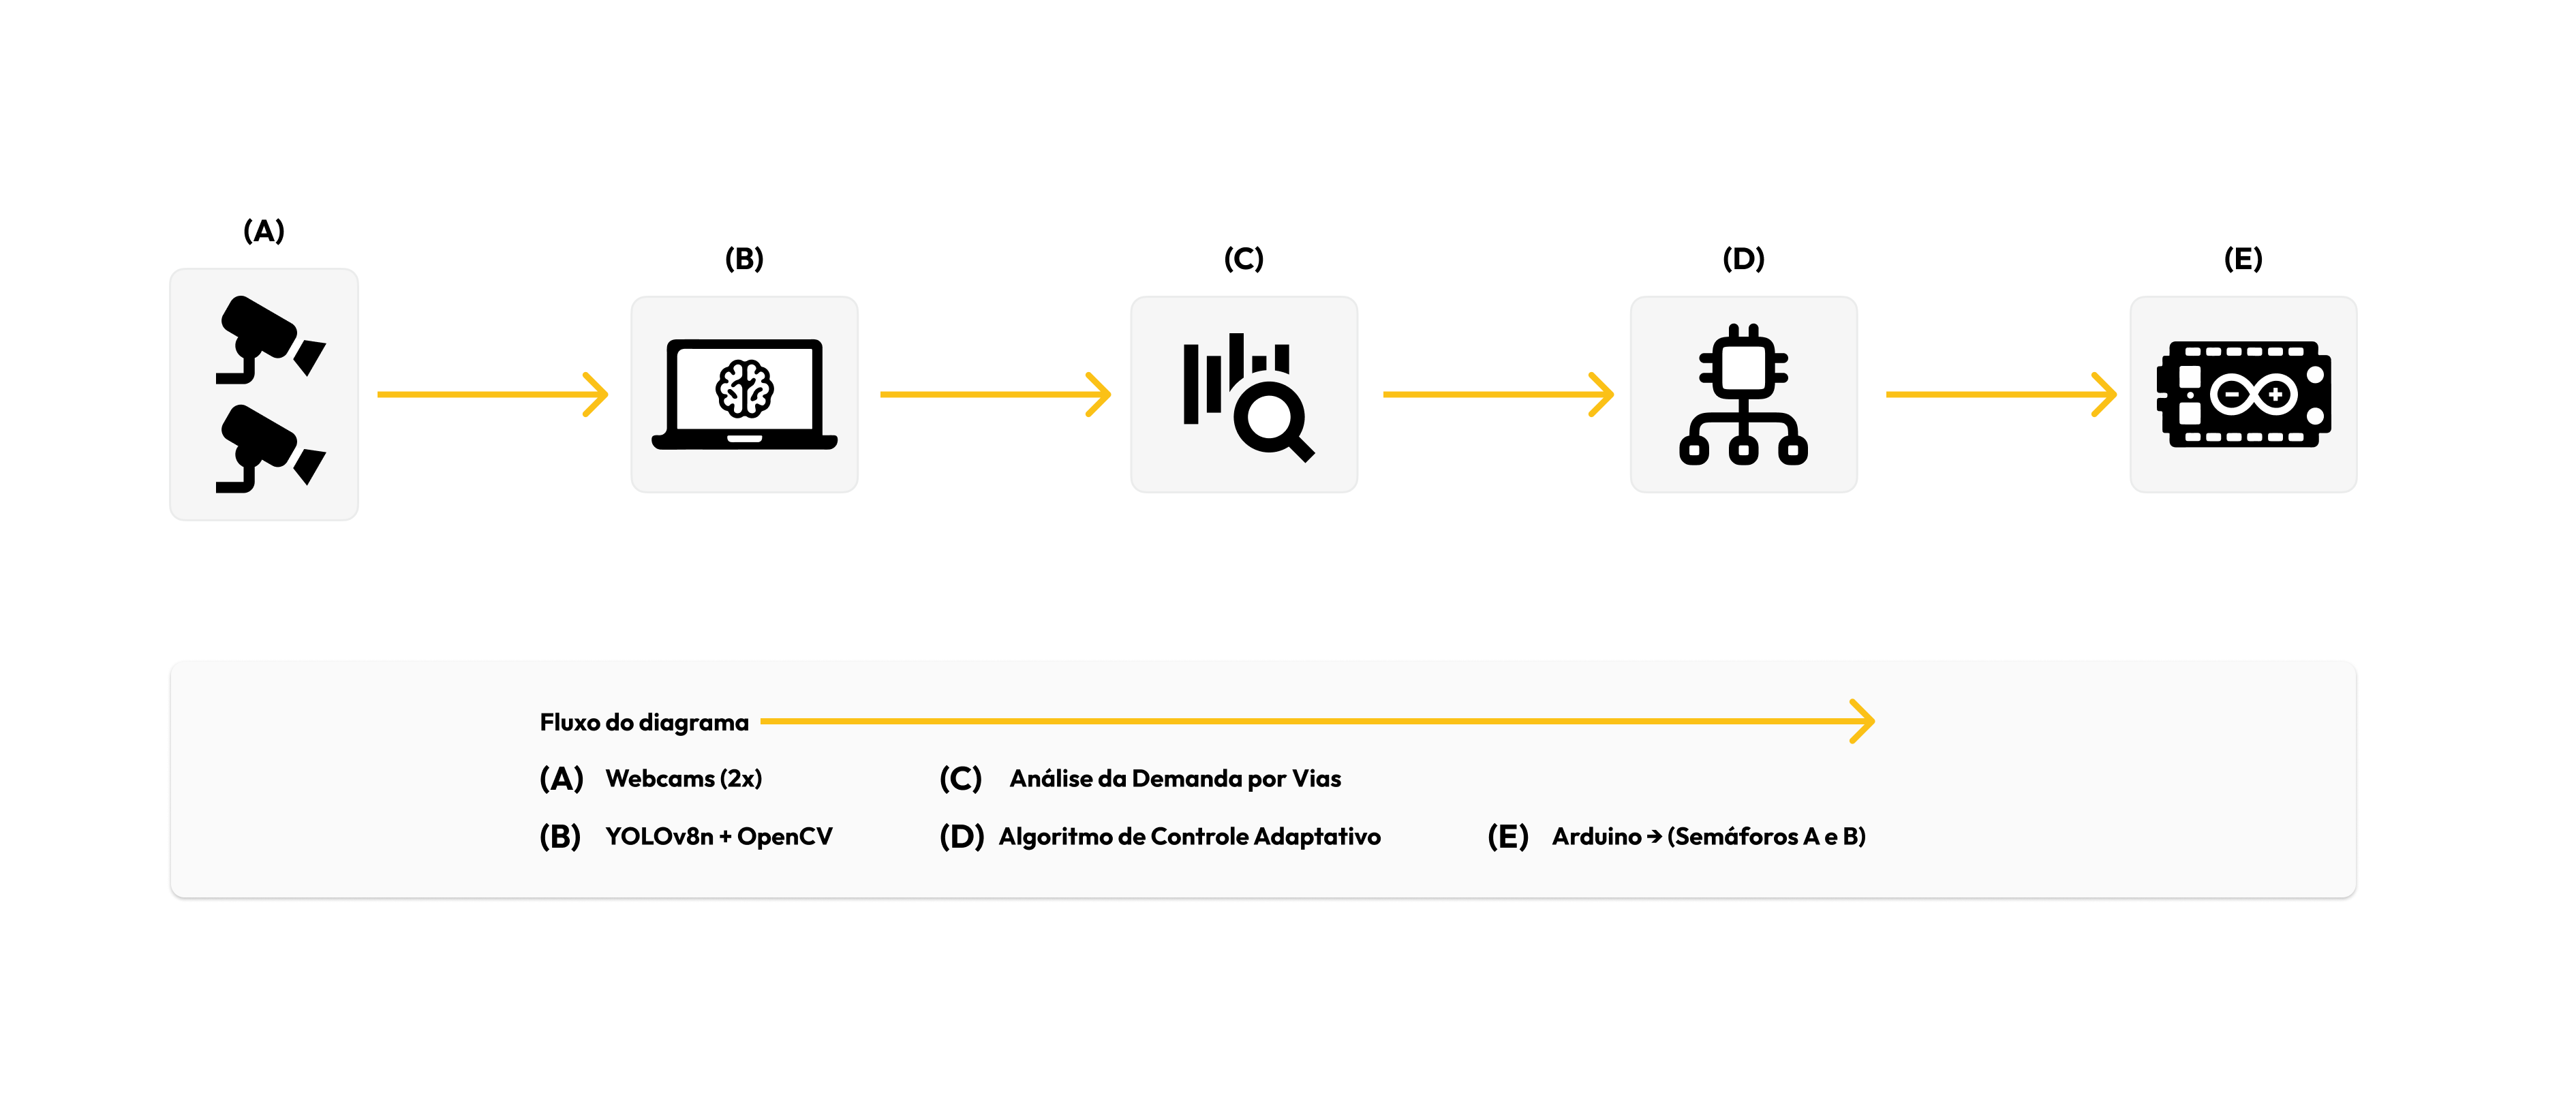
\includegraphics[width=\textwidth]{imgs/diagrama-de-rede-v3.png}
\caption{Diagrama de Infraestrutura do Sistema -- V3}
\label{fig:infra-v3}
\end{figure}

\begin{figure}[H]
\centering
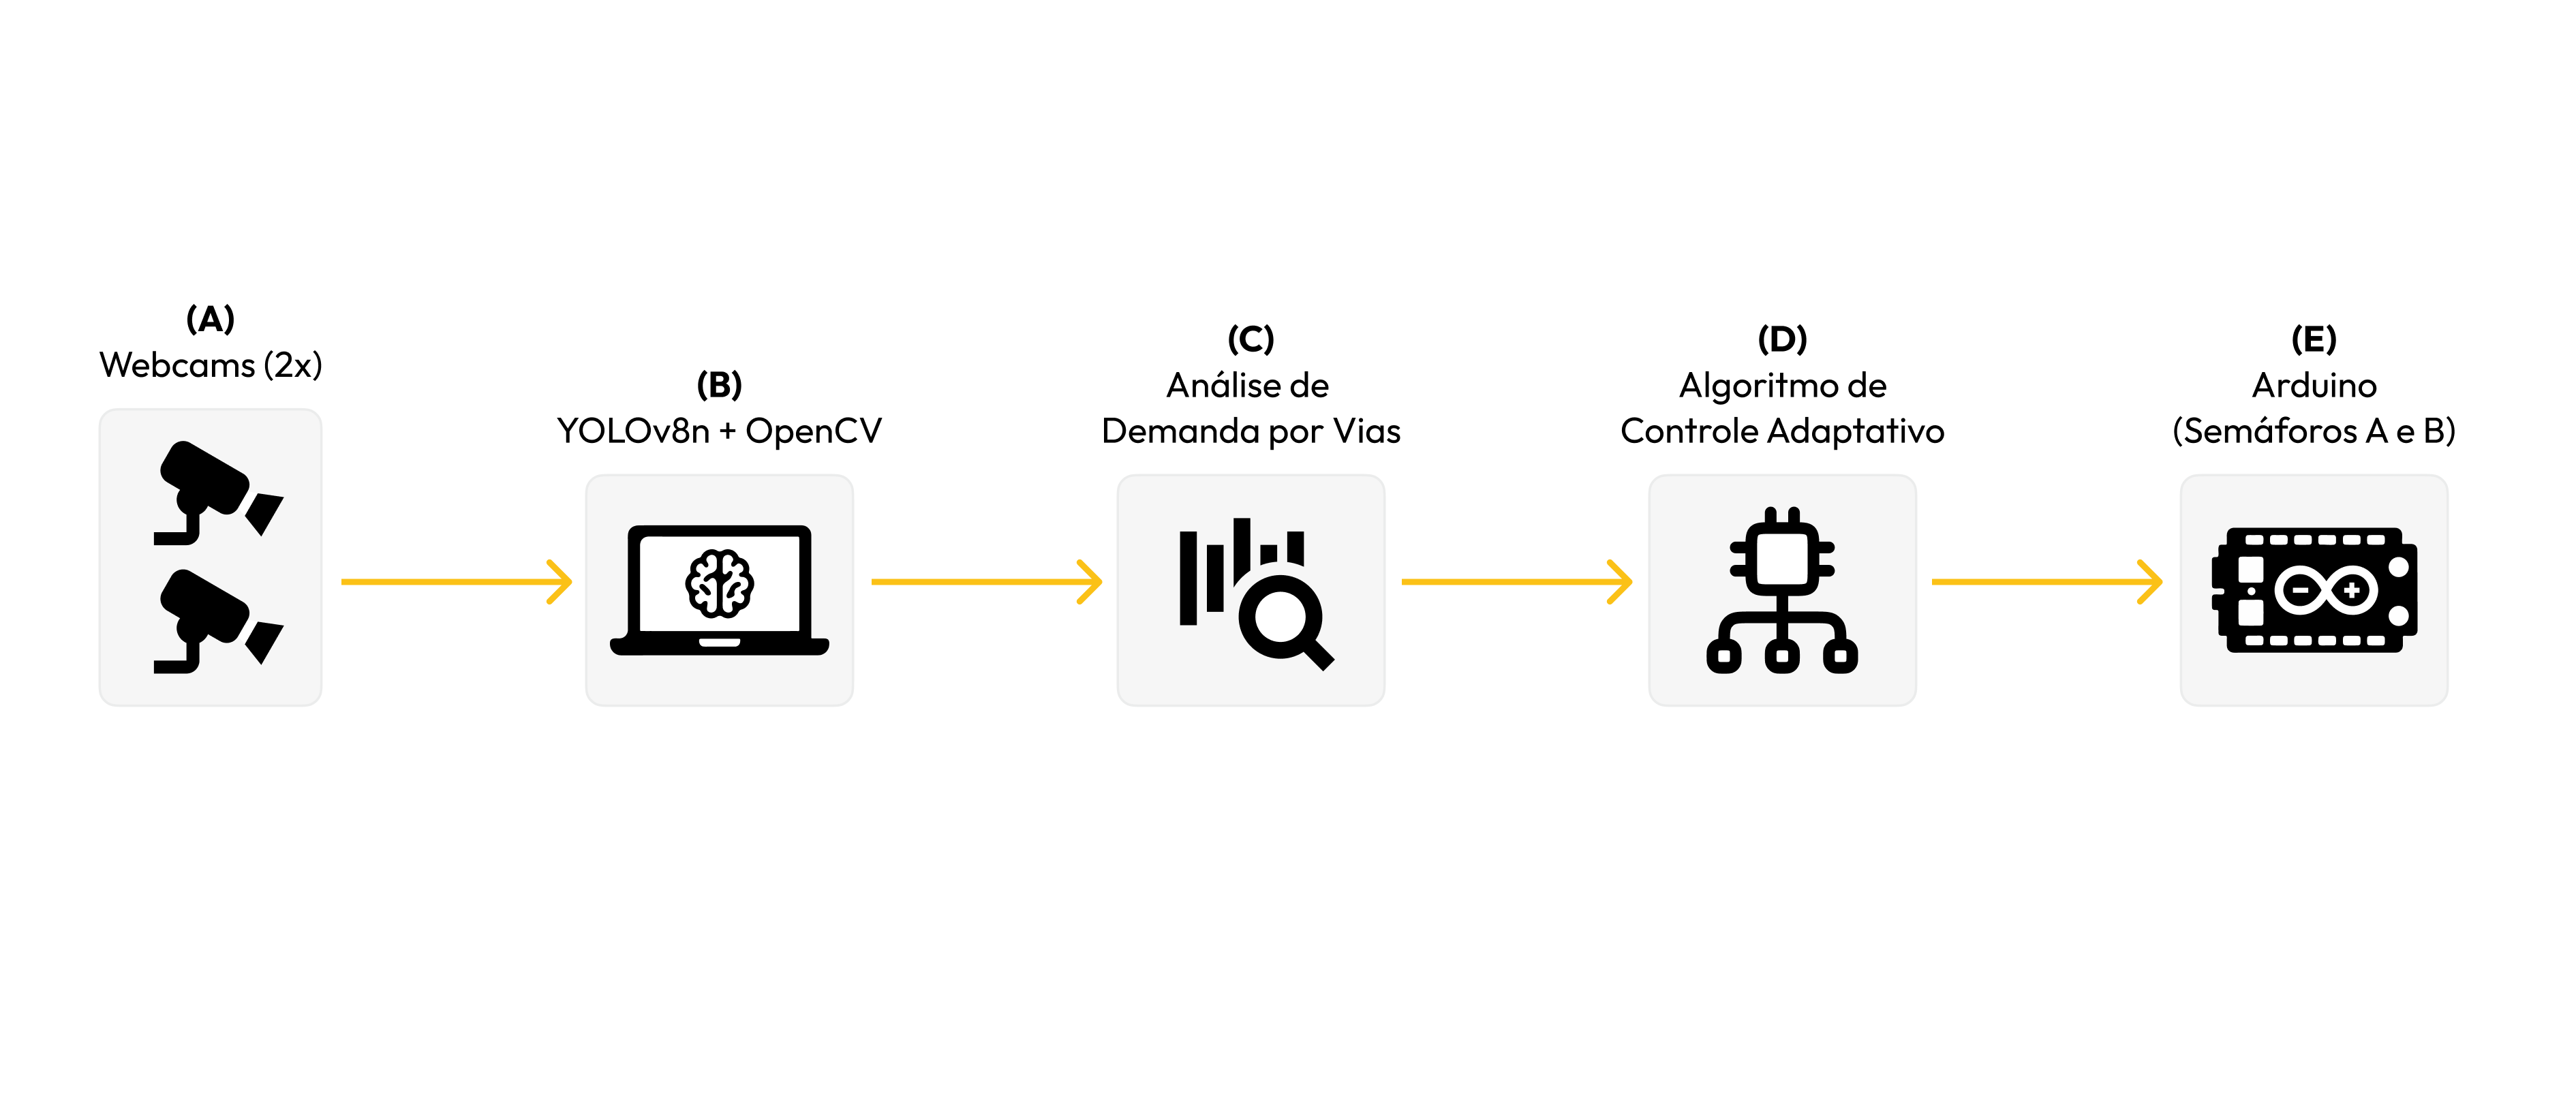
\includegraphics[width=\textwidth]{imgs/diagrama-de-rede-v3-2.png}
\caption{Diagrama de Infraestrutura do Sistema -- V3.2}
\label{fig:infra-v4}
\end{figure}

% ===== DEVOPS =====
\section{DevOps: Infraestrutura, Automação e Entrega Contínua}

DevOps \cite{wang2023} é uma cultura e conjunto de práticas que integra desenvolvimento de software (Dev) e operações de TI (Ops), focando em automação, colaboração e entrega contínua.

\subsection{Pipeline CI/CD}

O pipeline de integração e entrega contínua é fundamental para automação:

\begin{figure}[H]
\centering
\begin{tikzpicture}[
    node distance=1.5cm,
    every node/.style={rectangle, draw, rounded corners, 
                       fill=secondarycolor!20, 
                       text width=2cm, 
                       align=center,
                       font=\small,
                       minimum height=1cm}
]
\node (code) {Code};
\node (build) [right of=code, xshift=1cm] {Build};
\node (test) [right of=build, xshift=1cm] {Test};
\node (deploy) [right of=test, xshift=1cm] {Deploy};
\node (monitor) [right of=deploy, xshift=1cm] {Monitor};

\draw[->, thick] (code) -- (build);
\draw[->, thick] (build) -- (test);
\draw[->, thick] (test) -- (deploy);
\draw[->, thick] (deploy) -- (monitor);
\draw[->, thick, dashed] (monitor) to[bend right=45] (code);
\end{tikzpicture}
\caption{Pipeline CI/CD}
\label{fig:cicd}
\end{figure}

\subsection{Exemplo de Configuração CI/CD}

Exemplo de arquivo \texttt{.gitlab-ci.yml} ou GitHub Actions:

\begin{verbatim}
stages:
  - build
  - test
  - deploy

build:
  stage: build
  script:
    - npm install
    - npm run build

test:
  stage: test
  script:
    - npm run test
    - npm run lint

deploy:
  stage: deploy
  script:
    - npm run deploy
  only:
    - main
\end{verbatim}

\subsection{Infraestrutura como Código}

\begin{table}[H]
\centering
\caption{Ferramentas DevOps Utilizadas}
\label{tab:devops-tools}
\begin{tabular}{|l|l|p{6cm}|}
\hline
\textbf{Categoria} & \textbf{Ferramenta} & \textbf{Finalidade} \\
\hline
Controle de Versão & Git + GitHub & Versionamento de código \\
CI/CD & GitHub Actions & Automação de build e deploy \\
Containerização & Docker & Empacotamento de aplicações \\
Orquestração & Kubernetes & Gerenciamento de containers \\
Monitoramento & Prometheus + Grafana & Métricas e dashboards \\
Logs & ELK Stack & Centralização de logs \\
IaC & Terraform & Provisionamento de infraestrutura \\
\hline
\end{tabular}
\end{table}

\subsection{Infraestrutura do Sistema}

Esta seção documenta como o sistema funciona em diferentes ambientes e plataformas.

\subsubsection{Arquitetura de Rede}

\begin{table}[H]
\centering
\caption{Componentes de Infraestrutura}
\label{tab:infrastructure}
\begin{tabular}{|l|p{10cm}|}
\hline
\textbf{Componente} & \textbf{Descrição} \\
\hline
\textbf{Rede Local (LAN)} & 
\begin{itemize}[leftmargin=*, nosep]
    \item Servidor local para desenvolvimento e testes
    \item Rede interna com IP fixo (ex: 192.168.1.x)
    \item Acesso via VPN para equipe remota
    \item Backup local diário em servidor dedicado
\end{itemize} \\
\hline
\textbf{Cloud (Nuvem)} & 
\begin{itemize}[leftmargin=*, nosep]
    \item Hospedagem em AWS/Azure/Google Cloud
    \item Auto-scaling para gerenciar demanda
    \item CDN para distribuição de conteúdo estático
    \item Backup automático em múltiplas regiões
    \item Ambiente de produção e homologação separados
\end{itemize} \\
\hline
\textbf{Dispositivos Móveis} & 
\begin{itemize}[leftmargin=*, nosep]
    \item API REST para comunicação mobile
    \item Suporte para iOS e Android
    \item Sincronização offline com cache local
    \item Push notifications para atualizações
    \item Responsive design para tablets
\end{itemize} \\
\hline
\textbf{Segurança} & 
\begin{itemize}[leftmargin=*, nosep]
    \item Firewall e SSL/TLS para comunicação segura
    \item Autenticação JWT e OAuth 2.0
    \item Criptografia de dados sensíveis
    \item Monitoramento de acessos e logs de auditoria
\end{itemize} \\
\hline
\end{tabular}
\end{table}


\subsection{Arquitetura de Deploy}

Para documentar a arquitetura de deployment:

\begin{figure}[H]
\centering
\begin{tikzpicture}[
    node distance=2cm,
    component/.style={rectangle, draw, rounded corners, 
                      fill=secondarycolor!20, 
                      text width=2.5cm, 
                      align=center,
                      minimum height=1.2cm}
]
\node[component] (lb) {Load Balancer};
\node[component, below left of=lb] (app1) {App Server 1};
\node[component, below right of=lb] (app2) {App Server 2};
\node[component, below of=app1, xshift=1.5cm] (db) {Database};
\node[component, below of=db] (cache) {Redis Cache};

\draw[<->, thick] (lb) -- (app1);
\draw[<->, thick] (lb) -- (app2);
\draw[<->, thick] (app1) -- (db);
\draw[<->, thick] (app2) -- (db);
\draw[<->, thick] (app1) -- (cache);
\draw[<->, thick] (app2) -- (cache);
\end{tikzpicture}
\caption{Arquitetura de Deployment}
\label{fig:deployment}
\end{figure}

\subsection{Métricas e SLA}

Definir métricas importantes para monitoramento:

\begin{itemize}
    \item \textbf{Disponibilidade:} 99.9\% (uptime)
    \item \textbf{Tempo de Resposta:} $<$ 200ms (média)
    \item \textbf{Taxa de Erro:} $<$ 0.1\%
    \item \textbf{Throughput:} 1000 requisições/segundo
    \item \textbf{Deploy Frequency:} Diário
    \item \textbf{Lead Time:} $<$ 1 hora
    \item \textbf{MTTR:} $<$ 30 minutos (Mean Time To Recovery)
\end{itemize}

\newpage
\section*{Conclusão}

Este documento apresenta os principais artefatos necessários para a documentação completa de um projeto de software. Cada seção fornece exemplos práticos de como inserir e formatar os diferentes tipos de artefatos utilizando \LaTeX.

Os artefatos documentados incluem:
\begin{itemize}
    \item \textbf{CANVAS:} Modelo de negócio e estratégia
    \item \textbf{SWOT:} Análise estratégica de forças, fraquezas, oportunidades e ameaças
    \item \textbf{UX/UI:} Design de interface e experiência do usuário
    \item \textbf{Website:} Estrutura e especificações técnicas web
    \item \textbf{Diagramas UML:} Modelagem visual do sistema
    \item \textbf{DevOps:} Infraestrutura, automação

\end{document}